\chapter{Aportaciones}

\section{Planificación}

Para el desarrollo de este proyecto, se ha requerido llevar a cabo una serie de tareas con diferentes dificultades e importancias. A continuación, se muestra una planificación general del mismo en la tabla \ref{tabla_planificación}, junto con las fases que componen su desarrollo, y una planificación temporal de cada apartado por separado,  (para obtener información adicional, véase el apéndice \ref{planificacion}). Cabe destacar que, cada apartado, se basa en los conocimientos adquiridos en los apartados anteriores, a la vez que introduce conceptos nuevos y mejora las prestaciones del modelo. De esta manera, cada apartado supondrá retos nuevos nunca antes vistos y, si un apartado anterior presenta algún fallo desconocido en el momento, se deberá volver a la etapa anterior y arreglarlo. Tras solventarlo, se podrá proseguir con la etapa posterior. Además, dada la naturaleza de `caja oscura' de las redes neuronales, estas presentan cierta dificultad a la hora de depurar el código. Por tanto, esto supondrá un tiempo de depuración considerable en todas y cada una de las implementaciones, tal y como se mostrará a continuación.

\begin{enumerate}[label=\textbullet]
	\item \textbf{Estudio previo}: Consiste en el estudio y comprensión de cuestiones generales, dentro del campo de aprendizaje automático y visión por computador, comunes a redes neuronales totalmente conectadas, y redes neuronales convolucionales.
	
	\item \textbf{Investigación y desarrollo de redes neuronales totalmente conectadas}: En este periodo, me centré en la investigación y comprensión sobre las redes neuronales totalmente conectadas a bajo nivel. De esta manera, sabía que podría generar cualquier tipo de red totalmente conectada de manera dinámica, sin necesidad de realizar ningún tipo de cálculo posterior, independientemente del lenguaje de programación empleado, así como del uso o no de librerías que faciliten el proceso. 
	
	\item \textbf{Investigación y desarrollo de redes neuronales convolucionales}:
	Una vez familiarizado con redes neuronales totalmente conectadas, se trató de comprender de igual forma las redes neuronales convolucionales, pues se encuentran ampliamente relacionadas.
	\item \textbf{Investigación y desarrollo de sistemas homogéneos con OpenMP}:
	
	Una vez, comprendido el funcionamiento tanto de las redes neuronales totalmente conectadas, como de las redes neuronales convolucionales, me centré en reducir los tiempos de cómputo requeridos en ellas, mediante un paralelismo orientado a datos con OpenMP, (se analizará en detalle en secciones posteriores).
	
	\item \textbf{Investigación y desarrollo de sistemas heterogéneos con CUDA y cuDNN}:
	Con el conocimiento teórico y práctico ya adquirido sobre sistemas homogéneos, aplicados tanto a redes neuronales totalmente conectadas como a redes neuronales convolucionales, se avanza ahora hacia la exploración de sistemas heterogéneos, aplicados a estas mismas arquitecturas de redes neuronales.
\end{enumerate}


\begin{table}[H]
	\centering
	\begin{tabular}{|lll|}
		\hline
		Apartado 	 &\vline  & Tiempo (Horas) \\
		\hline
		
		Estudio previo    & \vline & 16 \\			
		\hline
		Investigación y desarrollo  	 & \vline & 	\\
		de redes neuronales  	 & \vline & 143	\\
		totalmente conectadas 	 & \vline & 	\\
		\hline
		Investigación y desarrollo    & \vline & 	 \\	
		de redes neuronales    & \vline & 152	 \\			
		convolucionales    & \vline & 	 \\					
		\hline
		Investigación y desarrollo  	 & \vline & 	 \\
		de sistemas homogéneos  	 & \vline & 103	 \\
		con OpenMP 	 & \vline & 	 \\
		\hline
		Investigación y desarrollo     & \vline &  	\\
		de sistemas heterogéneos    & \vline &  \\ 
		con CUDA y cuDNN    & \vline & 282 \\ 	
		\hline
		\hline
		Tiempo total:				& \vline & 696 \\
		\hline
	\end{tabular}
	\caption{Planificación del proyecto}
	\label{tabla_planificación}
\end{table}

\section{Retropropagación en redes neuronales rotalmente conectadas}

En esta sección, se analizará en profundidad el cálculo del gradiente de la pérdida con respecto a cada parámetro entrenable de una red totalmente conectada, así como con respecto a la entrada y salida de cada capa. Primero, se presentarán los cálculos para ejemplos concretos, y, una vez comprendidas las bases, se mostrará cómo aplicarlos a cualquier tipo de red totalmente conectada.

\subsection{Retropropagación en capa SoftMax} 

Tal y como se comentó en secciones anteriores, se empleará SoftMax en la última capa totalmente conectada. De este modo, se definen los valores de entrada a la misma como \textit{Z}, y los de salida como \textit{O}, tal y como se muestra en la Figura \ref{cross_entropy_notacion}.

\begin{figure}[H]
	\centering
	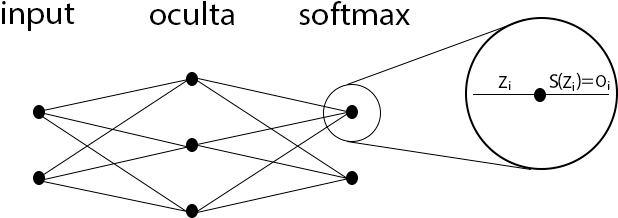
\includegraphics[scale=0.4]{imagenes/NN_softmax.jpg}  
	\caption{Estructura de una red totalmente conectada con softmax en la última capa}
\end{figure}

Según esta notación, la función de error \ref{fig:loss_func_softmax} se convierte en la fórmula \ref{cross_entropy_notacion}.

\begin{gather}
	E = - \sum_{i=1}^{N}  [y_i * ln(O_i)] 
	\label{cross_entropy_notacion}
\end{gather}

De este modo, se define el cálculo del gradiente de la pérdida, con respecto a cada neurona de entrada $Z_k$, de la capa SoftMax, según la fórmula \ref{gradiente_softmax} \cite{Cross_entropy_backprop} \cite{Cross_entropy_backprop_grad_input}. Para obtener una explicación detallada, y un desarrollo completo sobre los orígenes de dicha fórmula, consulte el apéndice \ref{softmax_apendice}.

\begin{gather}
	\frac{\partial E}{\partial Z_k} = O_k - y_k = gradiente\_Z_k
	\label{gradiente_softmax}
\end{gather}

\subsection{Retropropagación con 1 capa oculta \cite{NN_backpropagation} \cite{NN_backprop_2} \label{backprop_1_capa}}

En esta sección, se tratará de calcular el gradiente de la pérdida con respecto a cada parámetro de la red totalmente conectada, mostrada en la Figura \ref{fig:nn_1_capa}. Para no repetir cálculos, en esta y secciones posteriores, no se volverá a calcular la retropropagación a través de la capa SoftMax, pues los cálculos son siempre los mismos por ser la última capa de la arquitectura.

\begin{figure}[H]
	\centering
	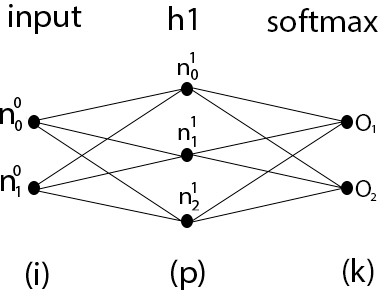
\includegraphics[scale=0.35]{imagenes/nn_1_capa.jpg}  
	\caption{Red Neuronal totalmente conectada con 1 capa oculta}
	\label{fig:nn_1_capa}
\end{figure}

La Figura \ref{fig:nn_1_capa} se compone de 'puntos' interconectados mediante líneas, representando estos neuronas y pesos que las conectan respectivamente. Cada punto corresponde a una neurona, y cada línea a un peso. \\
La Figura \ref{fig:nn_1_capa} presenta 3 capas (input, h1, softmax), que corresponden a la capa de entrada, la capa oculta $h_1$, y la capa de salida, respectivamente. El superíndice indica la capa a la que pertenece una neurona o peso, mientras que el subíndice indica el número del mismo en su respectiva capa. En el caso de los pesos, se requieren 2 subíndices para identificar a cada uno, (cada peso une 2 neuronas). \\
De esta manera, la capa de entrada se compone de 2 neuronas ($n^{0}_0$ y $n^{0}_1$), la capa oculta $h_1$ tiene 3 neuronas ($n^1_{0}$, $n^1_{1}$, y $n^1_{2}$), y el peso $W^{i}_{jk}$ referencia al peso que une las neuronas $n^{i}_j$ y $n^{i+1}_k$.\\
De forma adicional, se recuerda que $Z_i$ representa la entrada $i$ de la capa SoftMax, y, $O_i$, su salida.  

\subsubsection{Capa SoftMax}

\begin{figure}[H]
	\centering
	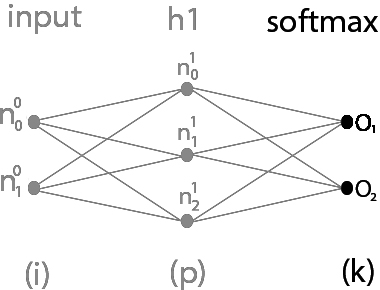
\includegraphics[scale=0.35]{imagenes/nn_1_capa_output.jpg}  
	\caption{Retropropagación en la capa softmax}
	\label{fig:nn_1_capa_output}
\end{figure}

Sea la neurona $n^i_j$, se define como $a^i_j$ el valor de dicha neurona antes de aplicar sobre ella su función de activación asociada, y, $z^i_j$, el obtenido tras aplicarla. 

Tal y como se calculó previamente, el gradiente de la función de pérdida con respecto a cada $Z_i$ viene dado por la fórmula \ref{gradiente_softmax}.


\subsubsection{Pesos capas h1-SoftMax}

\begin{figure}[H]
	\centering
	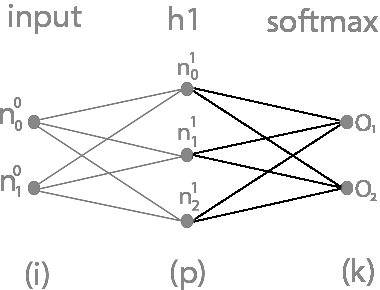
\includegraphics[scale=0.35]{imagenes/nn_1_capa_pesos_h1_output.jpg}  
	\caption{Retropropagación con respecto a pesos entre la capa oculta y la capa SoftMax}
	\label{fig:nn_1_pesos_h1_output}
\end{figure}

Una vez obtenido el gradiente hasta la entrada de la capa softmax, se puede calcular el gradiente con respecto a cada peso $W^1_{pk}$, pues se encuentra conectado a esta desde la capa anterior. Es decir, para cada $h^1_p\in h_1$, se calcula $\frac{dE(x)}{dW^1_{pk}}$. Usando la regla de la cadena, equivale a realizar lo ilustrado en las fórmulas \ref{grad_w1pk_1} y \ref{grad_w1pk_2}.

\begin{gather}
	\frac{\partial Z_k}{\partial W^1_{pk}} = \frac{\partial (z^1_p * W^1 _{pk}+ b^2_k)}{\partial W^1_{pk }} = z^1_p
	\label{grad_w1pk_1}
\end{gather}

\begin{gather}
	\frac{\partial E(x)}{\partial W^1_{pk }} =  gradiente\_Z_k * \frac{\partial Z_k}{\partial W^1_{pk }} = gradiente\_Z_k * z^1_p
	\label{grad_w1pk_2}
\end{gather}

\subsubsection{Sesgos capa softmax}

Del mismo modo, se calcula el gradiente de la pérdida con respecto a cada sesgo de las neuronas de la capa softmax, tal y como se muestra en las fórmulas \ref{grad_b_h1_1}, \ref{grad_b_h1_2} y \ref{grad_b_h1_3}.

\begin{gather}
	\frac{\partial E}{\partial b^2_k} = \frac{\partial E}{\partial Z_k} * \frac{\partial Z_k}{b^2_k} \label{grad_b_h1_1} \\
	\frac{\partial Z_k }{\partial b^2_k } = \frac{\partial ([\sum_{c=1}^{P} z^1_c * W^1_{pk}] + b^2_k) }{\partial b^2_k } = 1 \label{grad_b_h1_2} \\
	\frac{\partial E}{\partial b^2_k} = gradiente\_Z_k \label{grad_b_h1_3}
\end{gather}

\subsubsection{Capa oculta h1}

\begin{figure}[H]
	\centering
	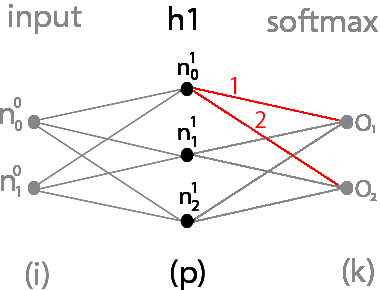
\includegraphics[scale=0.35]{imagenes/nn_caminos_posibles.jpg}  
	\caption{Imagen de los 'caminos' desde la capa softmax hasta la neurona $n^1_0$}
	\label{nn_caminos_posibles}
\end{figure}

En la figura \ref{nn_caminos_posibles}, se muestra como hay más de un 'camino' desde la capa softmax hasta $n^1_p$. Por lo tanto, para obtener el gradiente de la pérdida con respecto a $n^1_p$, es necesario calcular la suma de todos los 'caminos' hacia este, tal y como se presenta en las fórmulas \ref{E_total_a1p} y \ref{deriv_Zk_z1p}. \\

\begin{gather}
	\frac{\partial E_{total}}{\partial a^1_p} = \sum_{k=1}^K \frac{\partial E_k}{\partial a^1_p} = \sum_{k=1}^K  gradiente\_Z_k * \frac{\partial Z_k}{\partial z^1_p} * \frac{\partial z^1_p}{\partial a^1_p}
	\label{E_total_a1p}
\end{gather}

\begin{gather}
	\frac{\partial Z_k}{\partial z^1_p} = \frac{\partial( [\sum_{c=1}^{P} z^1_c * W^1_{ck}] + b^2_k)}{\partial z^1_p} = W^1_{pk}
	\label{deriv_Zk_z1p}
\end{gather}

Para calcular dichos gradientes, se requiere calcular $\frac{\partial z^1_p}{\partial a^1_p}$. Como se mencionó anteriormente, ``a'', se refiere al valor de una neurona antes de aplicar su función de activación asociada, y, ``z'', al valor obtenido tras su aplicación. Por lo tanto, para calcular $\frac{\partial z^1_p}{\partial a^1_p}$, se requiere conocer dicha función de activación.

\begin{figure}[H]
	\centering
	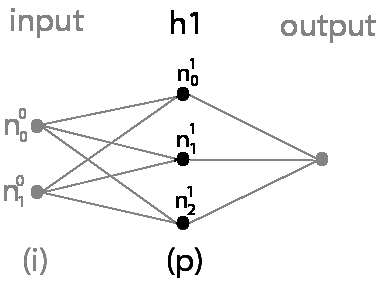
\includegraphics[scale=0.35]{imagenes/nn_1_capa_h1.jpg}  
	\caption{Retropropagación con respecto a neuronas de la capa oculta h1}
	\label{fig:nn_1_capa_h1}
\end{figure}

En este ejemplo, en la capa oculta h1 se emplea la función de activación sigmoide, y su derivada viene dada por las fórmulas \ref{grad_sig_1} y \ref{grad_sig_2}. 

\begin{gather}
	sigmoide(x) = \frac{1}{1+e^{-x}} \label{grad_sig_1} \\
	sigmoide'(x) = \frac{sigmoide(x)}{1-sigmoide(x)} \label{grad_sig_2}
\end{gather}

De este modo, ahora sí se puede calcular $\frac{\partial z^1_p}{\partial a^1_p}$, y se muestra en la fórmula \ref{deriv_z1p_a1p}.

\begin{gather}
	\frac{\partial z^1_ p}{\partial a^1_p} = \frac{\partial sigmoide(a^1_p)}{\partial a^1_p} = sigmoide(a^1_p)*(1-sigmoide(a^1_p))
	\label{deriv_z1p_a1p}
\end{gather}

Así, se retoma la fórmula \ref{E_total_a1p} mediante la aplicación de \ref{deriv_Zk_z1p} y \ref{deriv_z1p_a1p}, y se obtiene \ref{grad_E_a1p}.

\begin{gather}
	\frac{\partial E_{total}}{\partial a^1_p} = \sum_{k=1}^K  gradiente\_Z_k * W^1_{pk} * sigmoide(a^1_p)*(1-sigmoide(a^1_p)) \label{grad_E_a1p} \\
	\frac{\partial E_{total}}{\partial a^1_p} = gradiente\_h1_p
\end{gather}

\subsubsection{Pesos capas entrada-h1}

Una vez realizada la retropropagación hasta las neuronas de entrada de la capa oculta h1, se puede continuar con el proceso hacia la capa anterior, es decir, la capa de entrada.

\begin{figure}[H]
	\centering
	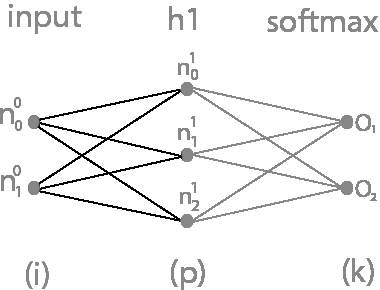
\includegraphics[scale=0.35]{imagenes/nn_1_capa_pesos_input_h1.jpg}  
	\caption{Retropropagación con respecto a los pesos entre la capa de entrada y la capa oculta h1}
	\label{fig:nn_1_pesos_input_h1}
\end{figure}


\begin{gather}
	\frac{\partial a^1_p }{\partial W^0_{ip} } = \frac{\partial [\sum_{c=1}^{I} z^0_c * W^0_{cp}] + b^1_p)}{\partial W^0_{ip} } = z^0_i \label{grad_w0ip_1} \\
	\frac{\partial E}{\partial W^0_{ip}} = \frac{\partial E_{total} }{\partial a^1_p } * \frac{\partial a^1_p}{W^0_{ip}} \label{grad_w0ip_2} \\
	\frac{\partial E(x) }{\partial W^0_{ip} } = gradiente\_h1_p * \frac{\partial a^1_p }{\partial W^0_{ip} } = gradiente\_h1_p * z^0_i 
	\label{grad_w0ip_3}
\end{gather}

De manera similar a como se calcularon los gradientes de la pérdida con respecto a los pesos entre la capa oculta $h_1$ y la capa softmax, se calcula el gradiente de la pérdida con respecto a los pesos entre la capa de entrada y la capa oculta h1. Este proceso se detalla en las fórmulas \ref{grad_w0ip_1}, \ref{grad_w0ip_2}, y \ref{grad_w0ip_3}.

\subsubsection{Sesgos capa h1}

\begin{gather}
	\frac{\partial E}{\partial b^1_p} = \frac{\partial E_{total} }{\partial a^1_p } * \frac{\partial a^1_p}{b^1_p} \label{grad_b1p_1} \\
	\frac{\partial a^1_p }{\partial b^1_p } = \frac{\partial ([\sum_{c=1}^{I} z^0_c * W^0_{ip}] + b^1_p) }{\partial b^1_p } = 1 \label{grad_b1p_2} \\
	\frac{\partial E}{\partial b^1_p} = gradiente\_h1_p
	\label{grad_b1p_3}
\end{gather}

De manera similar, las figuras \ref{grad_b1p_1}, \ref{grad_b1p_2}, y \ref{grad_b1p_3} ilustran el cálculo del gradiente con respecto a los sesgos de la capa oculta h1.

\subsubsection{Capa de entrada}

\begin{figure}[H]
	\centering
	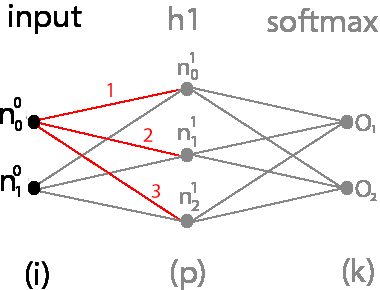
\includegraphics[scale=0.35]{imagenes/nn_caminos_posibles_input.jpg}  
	\caption{Imagen de los 'caminos' desde la capa oculta h1 hasta $n^0_0$}
	\label{nn_caminos_posibles_input}
\end{figure}

Por último, en esta sección se calcula el gradiente con respecto a las neuronas de entrada de la capa de entrada. Aunque, en general, no sería necesario calcular estos gradientes, dado que el objetivo es construir una red neuronal convolucional (CNN), es imprescindible hacerlo. Esto se debe a que la red totalmente conectada estará integrada con capas convolucionales y de agrupación máxima, por lo que es necesario calcular estos gradientes para poder continuar con el proceso de retropropagación en las capas anteriores a esta.

\begin{gather}
	\frac{\partial E_{total}}{\partial a^0_i} = \sum_{p=1}^P \frac{\partial E_{total}}{\partial a^1_p} * \frac{\partial a^1_p}{\partial z^0_i} * \frac{\partial z^0_i}{\partial a^0_i} \label{grad_a_1} \\
	\frac{\partial a^1_p }{\partial z^0_i } = \frac{\partial ([\sum_{c=1}^{I} z^0_c * W^0_{ip}] + b^1_p) }{\partial z^0_i } = W^0_{ip} \label{grad_a_2}
\end{gather}

\begin{figure}[H]
	\centering
	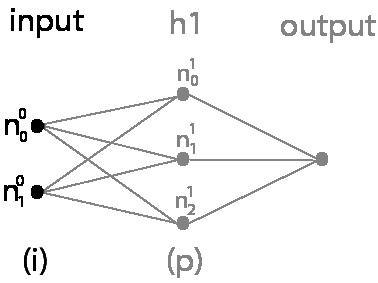
\includegraphics[scale=0.35]{imagenes/nn_1_capa_input.jpg}  
	\caption{Retropropagación en la capa input}
	\label{fig:nn_1_capa_input}
\end{figure}

Como la capa input no presenta ninguna función de activación asociada, se tiene que $z^0_i$ es igual $a^0_i$. \\

\begin{gather}
	\frac{\partial z^0_i }{\partial a^0_i } = 1 \\
	\frac{\partial E_{total}}{\partial a^0_i} = \sum_{p=1}^{P} gradiente\_h1_p
\end{gather}

\subsection{Retropropagación con 2 capas ocultas}

\begin{figure}[H]
	\centering
	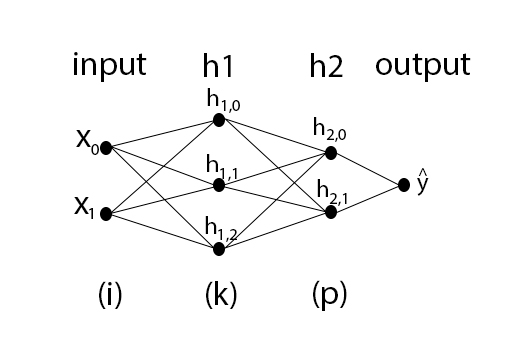
\includegraphics[scale=0.35]{imagenes/nn_2_capas.jpg}  
	\caption{Red Neuronal totalmente conectada con 2 capas ocultas}
	\label{fig:nn_2_capas}
\end{figure}

A diferencia del apartado anterior, en este caso se utiliza una red totalmente conectada con 2 capas ocultas (h1 y h2), tal y como se muestra en la Figura \ref{fig:nn_2_capas}. \\

\subsubsection{Capa SoftMax}

\begin{figure}[H]
	\centering
	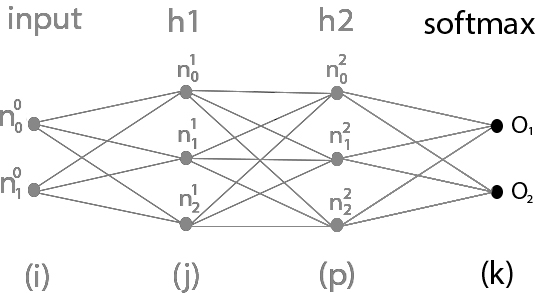
\includegraphics[scale=0.35]{imagenes/nn_2_capa_output.jpg}  
	\caption{Retropropagación en la capa softmax}
\end{figure}

De manera similar a los casos anteriores, el gradiente de la función de pérdida con respecto a cada $Z_i$, se determina mediante la fórmula \ref{gradiente_softmax}. En consecuencia, no se repetirá el cálculo. \\

\subsubsection{Pesos capas h2-SoftMax}

\begin{figure}[H]
	\centering
	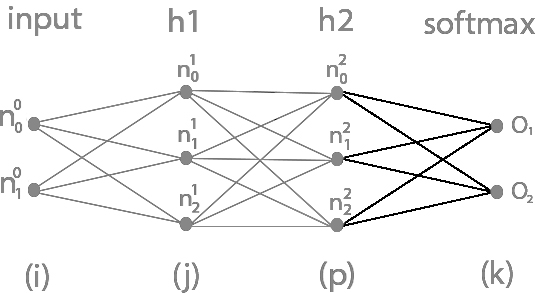
\includegraphics[scale=0.35]{imagenes/nn_2_capa_pesos_h2_output.jpg}  
	\caption{Retropropagación respecto a los pesos entre la capa oculta h2 y la capa SoftMax}
	\label{fig:nn_2_capa_pesos_h2_output}
\end{figure}

Se lleva a cabo el cálculo del gradiente de la función de pérdida con respecto a cada peso $W^2_{pk}$ que conecta las neuronas de la capa oculta h2 con las de la capa softmax (véase la figura \ref{fig:nn_2_capa_pesos_h2_output}). \\

\begin{gather}
	\frac{\partial Z_k}{\partial W^2_{pk}} = \frac{\partial (z^2_p * W^2 _{pk} + b^3_k)}{\partial W^2_{pk }} = z^2_p 
	\label{grad_w2pk_1}
\end{gather}

\begin{gather}
	\frac{\partial E(x)}{\partial W^2_{pk }} =  gradiente\_Z_k * \frac{\partial Z_k}{\partial W^2_{pk }} = gradiente\_Z_k * z^2_p
	\label{grad_w2pk_2}
\end{gather}

Como era de esperar, las fórmulas \ref{grad_w2pk_1} y \ref{grad_w2pk_2} son prácticamente idénticas a las fórmulas \ref{grad_w1pk_1} y \ref{grad_w1pk_2}, respectivamente, con la única diferencia del superíndice empleado (1 $\neq$ 2). Esto resulta lógico, ya que esta parte del cálculo es también común al apartado anterior.

\subsubsection{Sesgos capa softmax}

\begin{gather}
	\frac{\partial E}{\partial b^3_k} = \frac{\partial E}{\partial Z_k} * \frac{\partial Z_k}{b^3_k} \label{grad_b_h2_1} \\
	\frac{\partial Z_k }{\partial b^3_k } = \frac{\partial ([\sum_{c=1}^{P} z^2_c * W^2_{pk}] + b^3_k) }{\partial b^3_k } = 1 \label{grad_b_h2_2} \\
	\frac{\partial E}{\partial b^3_k} = gradiente\_Z_k \label{grad_b_h2_3}
\end{gather}

De manera similar, el cálculo del gradiente de la pérdida con respecto a los sesgos de la capa softmax también se mantiene inalterado. Por consiguiente, la única diferencia entre las fórmulas $\{$\ref{grad_b_h2_1}, \ref{grad_b_h2_2}, \ref{grad_b_h2_3}$\}$ y $\{$\ref{grad_b_h1_1}, \ref{grad_b_h1_2}, \ref{grad_b_h1_3}$\}$ radica en los superíndices utilizados.

\subsubsection{Capa oculta h2}

\begin{figure}[H]
	\centering
	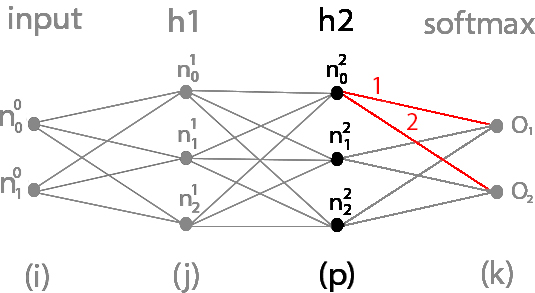
\includegraphics[scale=0.35]{imagenes/nn_h2_caminos_posibles.jpg}  
	\caption{Imagen de los 'caminos' desde la capa softmax hasta $n^2_0$}
	\label{nn_h2_caminos_posibles}
\end{figure}

Tal y como se comentó anteriormente, existen mútiples 'caminos' desde la capa softmax hasta $n^2_p$. Por lo tanto, para obtener el gradiente de la pérdida con respecto a cada $n^2_p$, es necesario calcular la suma de todos ellos, tal y como se detalla en las fórmulas \ref{E_total_a2p} y \ref{deriv_Zk_z2p}. \\

\begin{gather}
	\frac{\partial E_{total}}{\partial a^2_p} = \sum_{k=1}^K \frac{\partial E_k}{\partial a^2_p} = \sum_{k=1}^K  gradiente\_Z_k * \frac{\partial Z_k}{\partial z^2_p} * \frac{\partial z^2_p}{\partial a^2_p}
	\label{E_total_a2p}
\end{gather}

\begin{gather}
	\frac{\partial Z_k}{\partial z^2_p} = \frac{\partial( [\sum_{c=1}^{P} z^2_c * W^2_{ck}] + b^3_k)}{\partial z^2_p} = W^2_{pk}
	\label{deriv_Zk_z2p}
\end{gather}

\begin{figure}[H]
	\centering
	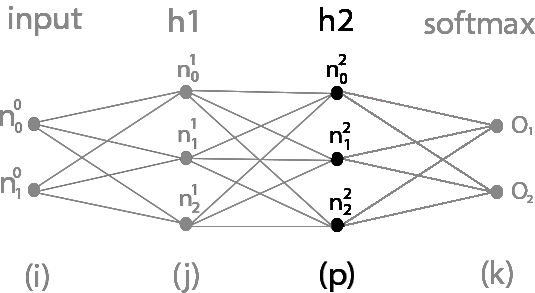
\includegraphics[scale=0.35]{imagenes/nn_2_capa_h2.jpg}  
	\caption{Retropropagación en la capa oculta h2}
	\label{fig:nn_2_capa_h2}
\end{figure}

Dado que coincide con el ejemplo anterior, en la última capa oculta (en este caso, h2), se utiliza nuevamente la función de activación sigmoide. Por lo tanto, se reitera la derivada de esta función en las fórmulas \ref{grad_sig_h2_1} y \ref{grad_sig_h2_2} para facilitar la comprensión del lector.

\begin{gather}
	sigmoide(x) = \frac{1}{1+e^{-x}} \label{grad_sig_h2_1} \\
	sigmoide'(x) = \frac{sigmoide(x)}{1-sigmoide(x)} \label{grad_sig_h2_2}
\end{gather}


Empleando la derivada de sigmoide, se obtiene la fórmula \ref{deriv_z2p_a2p}.

\begin{gather}
	\frac{\partial z^2_ p}{\partial a^2_p} = \frac{\partial sigmoide(a^2_p)}{\partial a^2_p} = sigmoide(a^2_p)*(1-sigmoide(a^2_p))
	\label{deriv_z2p_a2p}
\end{gather}

A continuación, se retoma la fórmula \ref{E_total_a2p} mediante la aplicación de \ref{deriv_Zk_z2p} y \ref{deriv_z2p_a2p} para obtener \ref{grad_E_a2p}.

\begin{gather}
	\frac{\partial E_{total}}{\partial a^2_p} = \sum_{k=1}^K  gradiente\_Z_k * W^2_{pk} * sigmoide(a^2_p)*(1-sigmoide(a^2_p)) \label{grad_E_a2p} \\
	\frac{\partial E_{total}}{\partial a^2_p} = gradiente\_h2_p
\end{gather}

Una vez más, la fórmula obtenida (\ref{grad_E_a2p}) coindice con la calculada previamente (\ref{grad_E_a1p}), salvo por los superíndices empleados. \\

\subsubsection{Pesos capas h1-h2}

\begin{figure}[H]
	\centering
	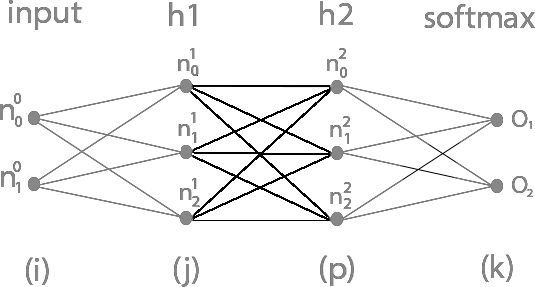
\includegraphics[scale=0.35]{imagenes/nn_2_capa_pesos_h1_h2.jpg}  
	\caption{Retropropagación respecto a los pesos entre las capas ocultas h1 y h2}
	\label{fig:nn_2_pesos_h1_h2}
\end{figure}


\begin{gather}
	\frac{\partial a^2_p }{\partial W^1_{jp} } = \frac{\partial [\sum_{c=1}^{J} z^1_c * W^1_{cp}] + b^2_p)}{\partial W^1_{jp} } = z^1_j \\
	\frac{\partial E}{\partial W^1_{jp}} = \frac{\partial E_{total} }{\partial a^2_p } * \frac{\partial a^2_p}{W^1_{jp}} \\
	\frac{\partial E(x) }{\partial W^1_{jp} } = gradiente\_h2_p * \frac{\partial a^2_p }{\partial W^1_{jp} } = gradiente\_h2_p * z^1_j 
	\label{grad_w1jp}
\end{gather}

Dado que esta parte también es común al caso anterior, la fórmula \ref{grad_w1jp} coincide nuevamente con la fórmula \ref{grad_w0ip_3}.


\subsubsection{Sesgos capa h2}

\begin{gather}
	\frac{\partial E}{\partial b^2_p} = \frac{\partial E_{total} }{\partial a^2_p } * \frac{\partial a^2_p}{b^2_p} \\
	\frac{\partial a^2_p }{\partial b^2_p } = \frac{\partial ([\sum_{c=1}^{J} z^1_c * W^1_{jp}] + b^2_p) }{\partial b^2_p } = 1 \\
	\frac{\partial E}{\partial b^2_p} = gradiente\_h2_p
	\label{grad_b2p}
\end{gather}

Una vez más, la fórmula \ref{grad_b2p} coincide con \ref{grad_b1p_3}. Es fundamental reconocer las partes comunes entre ambos casos, ya que esto facilita la generalización del modelo y la automatización de los cálculos correspondientes.

\subsubsection{Capa oculta h1}

\begin{figure}[H]
	\centering
	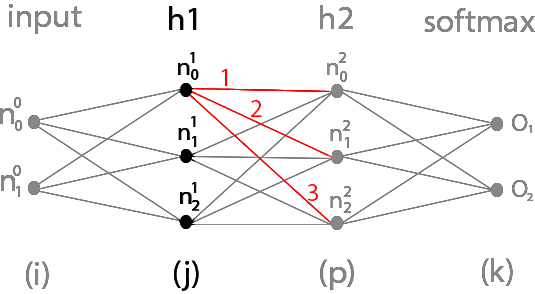
\includegraphics[scale=0.35]{imagenes/nn_h1_caminos_posibles.jpg}  
	\caption{'Caminos' desde la capa softmax hasta $n^1_0$}
	\label{nn_h1_caminos_posibles}
\end{figure}

De manera similar a lo realizado en la capa h2, se calcula la suma de todos los 'caminos' hacia cada neurona $n^1_j$. \\

\begin{gather}
	\frac{\partial E_{total}}{\partial a^1_j} = \sum_{k=1}^K \frac{\partial E_k}{\partial a^1_j} = \sum_{p=1}^P  gradiente\_h2_p * \frac{\partial a^2_p}{\partial z^1_j} * \frac{\partial z^1_j}{\partial a^1_j} \\
	\frac{\partial a^2_p}{\partial z^1_j} = \frac{\partial( [\sum_{c=1}^{J} z^1_c * W^1_{cp}] + b^2_p)}{\partial z^1_j} = W^1_{jp}
\end{gather}

Como era de esperar, se calcula el gradiente con respecto a cada neurona de la capa h1 considerando cada `camino' del gradiente proveniente la capa siguiente (h2).

\begin{figure}[H]
	\centering
	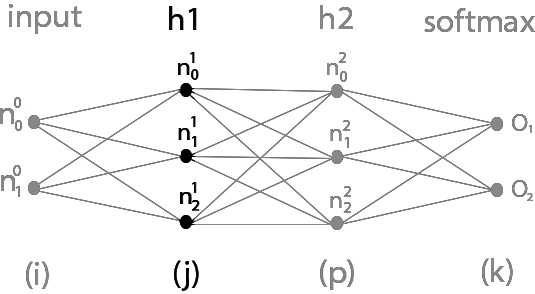
\includegraphics[scale=0.35]{imagenes/nn_2_capa_h1.jpg}  
	\caption{Retropropagación en la capa oculta h1}
\end{figure}

En este caso, en la capa oculta h1 se utiliza la función de activación ReLU, cuya derivada viene dada por la fórmula \ref{deriv_relu}. 

\begin{gather}
	ReLU(x) = max(0, x) \\
	ReLU'(x) = 1\ si\ x>0,\ 0\ en\ caso\ contrario
	\label{deriv_relu}
\end{gather}

La derivada la función de activación ReLU (fórmula \ref{label}), se emplea para obtener el gradiente $\frac{\partial z^1_ j}{\partial a^1_j}$, y para continuar con la retropropagación a través de la capa, tal y como se detalla en las fórmulas (\ref{grad_E_a1j_1}, \ref{grad_E_a1j_2}, y \ref{grad_E_a1j_3}).


\begin{gather}
	\frac{\partial z^1_ j}{\partial a^1_j} = 1\ si\ x>0,\ 0\ en\ caso\ contrario \label{grad_E_a1j_1} \\
	\frac{\partial E_{total}}{\partial a^1_j} = \sum_{p=1}^P  gradiente\_h2_p * W^1_{jp} * ReLU'(a^1_j) \label{grad_E_a1j_2} \\
	\frac{\partial E_{total}}{\partial a^1_j} = gradiente\_h1_j
	\label{grad_E_a1j_3}
\end{gather}

Una vez más, el proceso para obtener de la fórmula \ref{grad_E_a1j_2} es muy similar al utilizado en casos anteriores, a pesar de que pueda parecer relativamente nueva en comparación con la sección anterior. \\


\subsubsection{Pesos capa input-h1}

\begin{figure}[H]
	\centering
	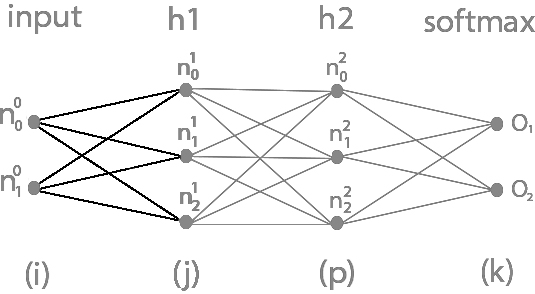
\includegraphics[scale=0.35]{imagenes/nn_2_capa_pesos_input_h1.jpg}  
	\caption{Retropropagación respecto a los pesos entre la capa de entrada y la capa oculta h1}
	\label{fig:nn_2_pesos_input_h1}
\end{figure}


\begin{gather}
	\frac{\partial a^1_j }{\partial W^0_{ij} } = \frac{\partial ([\sum_{c=1}^{I} z^0_c * W^0_{cj}] + b^1_j)}{\partial W^0_{ij} } = z^0_i \label{grad_w0ip_h2_1} \\
	\frac{\partial E}{\partial W^0_{ij}} = \frac{\partial E_{total} }{\partial a^1_j } * \frac{\partial a^1_j}{W^0_{ij}} \label{grad_w0ip_h2_2} \\
	\frac{\partial E(x) }{\partial W^0_{ij} } = gradiente\_h1_j * \frac{\partial a^1_j }{\partial W^0_{ij} } = gradiente\_h1_j * z^0_i \label{grad_w0ip_h2_3}
\end{gather}

Aquí se observa que las fórmulas $\{$\ref{grad_w0ip_h2_1}, \ref{grad_w0ip_h2_2}, \ref{grad_w0ip_h2_3} $\}$ son idénticas a $\{$\ref{grad_w0ip_1}, \ref{grad_w0ip_2}, \ref{grad_w0ip_3} $\}$, excepto por el subíndice empleado (j $\neq$ p). Aunque los valores analíticos puedan diferir debido a las diferencias en las arquitecturas, la notación utilizada se ha diseñado para facilitar la visualización y comprensión de la capacidad de automatización en las capas totalmente conectadas.

\subsubsection{Sesgos capa h1}

\begin{gather}
	\frac{\partial E}{\partial b^1_j} = \frac{\partial E_{total} }{\partial a^1_j } * \frac{\partial a^1_j}{b^1_j} \label{grad_b1j_h2_1} \\
	\frac{\partial a^1_j }{\partial b^1_j } = \frac{\partial ([\sum_{c=1}^{I} z^0_c * W^0_{ij}] + b^1_j) }{\partial b^1_j } = 1 \label{grad_b1j_h2_2} \\
	\frac{\partial E}{\partial b^1_j} = gradiente\_h1_j
	\label{grad_b1j_h2_3}
\end{gather}

De este modo, las fórmulas $\{$\ref{grad_b1j_h2_1}, \ref{grad_b1j_h2_2}, \ref{grad_b1j_h2_3} $\}$ y $\{$\ref{grad_b1p_1}, \ref{grad_b1p_2}, \ref{grad_b1p_3} $\}$ coinciden en todo los aspectos, excepto en el subíndice (j $\neq$ p).

\subsubsection{Capa input}

\begin{figure}[H]
	\centering
	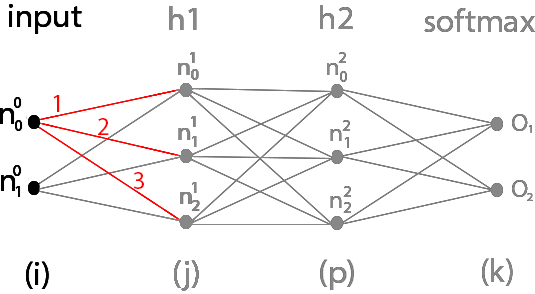
\includegraphics[scale=0.35]{imagenes/nn_2_capas_caminos_posibles_input.jpg}  
	\caption{'Caminos' desde la capa oculta h1 hasta $n^0_0$}
	\label{nn_2_capas_caminos_posibles_input}
\end{figure}

\begin{gather}
	\frac{\partial E_{total}}{\partial a^0_i} = \sum_{j=1}^J \frac{\partial E_{total}}{\partial a^1_j} * \frac{\partial a^1_j}{\partial z^0_i} * \frac{\partial z^0_i}{\partial a^0_i} \label{grad_a_h2_1} \\
	\frac{\partial a^1_j }{\partial z^0_i } = \frac{\partial ([\sum_{c=1}^{I} z^0_c * W^0_{ij}] + b^1_j) }{\partial z^0_i } = W^0_{ij} \label{grad_a_h2_2}
\end{gather}

Aquí también se observa que, a pesar de las diferencias en los subíndices utilizados, las fórmulas $\{$\ref{grad_a_h2_1}, \ref{grad_a_h2_2} $\}$ y $\{$\ref{grad_a_1}, \ref{grad_a_2}$\}$ son idénticas.

\begin{figure}[H]
	\centering
	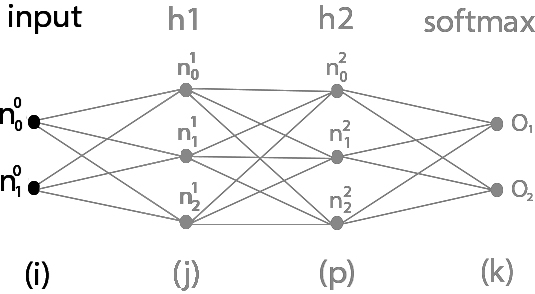
\includegraphics[scale=0.35]{imagenes/nn_2_capa_input.jpg}  
	\caption{Retropropagación en la capa input}
	\label{fig:nn_2_capa_input}
\end{figure}

Dado que la capa de entrada no tiene ninguna función de activación asociada, $z^0_i$ es igual $a^0_i$, al igual que en el caso anterior. \\

\begin{gather}
	\frac{\partial z^0_i }{\partial a^0_i } = 1 \\
	\frac{\partial E_{total}}{\partial a^0_i} = \sum_{p=1}^{P} gradiente\_h1_p
\end{gather}

\subsection{Conclusiones}
Se definen como capas ocultas ``intermedias'' todas las capas, exceptuando la última de ellas. Tal y como se ha demostrado anteriormente, estas capas comparten la mayoría de los cálculos asociados a la retropopagación. En consecuencia, una red neuronal totalmente conectada puede dividirse en 4 grupos $\{$capa de entrada, capas ocultas intermedias, última capa oculta, capa de salida o capa softmax$\}$. \\
A continuación se realiza el cálculo necesario para la retropropagación de una capa de neuronas \textit{l} específica. Suponemos que la capa \textit{l+1} tiene \textit{Q} neuronas, la capa \textit{l-1} tiene \textit{K} neuronas, y que todas las capas ocultas intermedias usan ReLU como función de activación. \\

\subsubsection{Gradiente respecto a la entrada de la capa}

\begin{figure}[H]
	\centering
	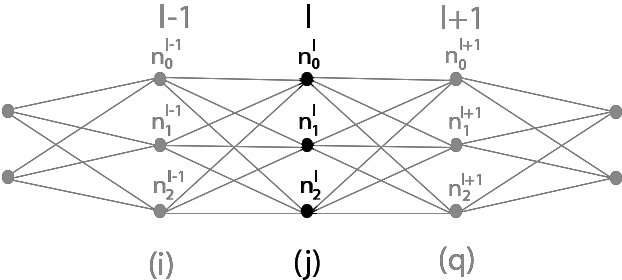
\includegraphics[scale=0.35]{imagenes/conclusion_capa_l.jpg}  
	\caption{Retropropagación en la capa l}
	\label{fig:conclusion_capa_l}
\end{figure}

\begin{gather}
	\frac{\partial E_{total}}{\partial a^l_j} = \sum_{q=1}^Q \frac{\partial E_{total}}{\partial a^{l+1}_q} * \frac{\partial a^{l+1}_q}{\partial z^l_j} * \frac{\partial z^l_j}{\partial a^l_j} \label{grad_input_l_1} \\
	\frac{\partial a^{l+1}_j }{\partial z^l_j } = \frac{\partial ([\sum_{c=1}^{K} z^l_c * W^l_{ij}] + b^{l+1}_j) }{\partial z^l_j } = W^l_{ij} \label{grad_input_l_2} \\
	\frac{\partial z^l_j}{\partial a^l_j} = ReLU'(a^l_j) \label{grad_input_l_3} \\
	\frac{\partial E_{total}}{\partial a^l_j} = \sum_{q=1}^Q  gradiente\_h_{{l+1}_q} * W^l_{ij} * ReLU'(a^l_j) \label{grad_input_l_4} \\
	\frac{\partial E_{total}}{\partial a^l_j} = gradiente\_h_{l_j} \label{grad_input_l_5}
\end{gather}

Las fórmulas \ref{grad_input_l_1}, \ref{grad_input_l_2}, \ref{grad_input_l_3},  \ref{grad_input_l_4}, y \ref{grad_input_l_5}, ilustran el cálculo genérico necesario para obtener el gradiente de la pérdida con respecto a la entrada de una capa oculta intermedia \textit{l}.

\subsubsection{Gradiente respecto a los pesos}

\begin{figure}[H]
	\centering
	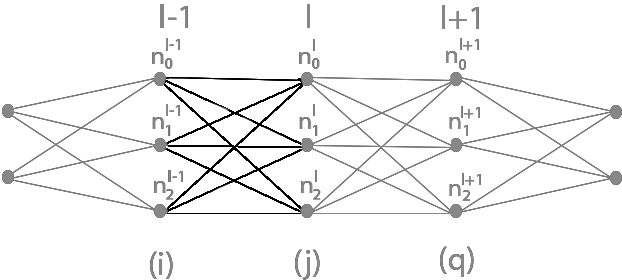
\includegraphics[scale=0.35]{imagenes/conclusion_pesos.jpg}  
	\caption{Retropropagación respecto a los pesos entre la capa l-1 y l}
	\label{fig:conclusion_pesos}
\end{figure}

\begin{gather}
	\frac{\partial E}{\partial W^{l-1}_{ij}} = \frac{\partial E_{total} }{\partial a^l_j } * \frac{\partial a^l_j}{W^{l-1}_{ij}} \label{grad_w_l_1} \\
	\frac{\partial a^l_j }{\partial W^{l-1}_{ij} } = \frac{\partial ([\sum_{c=1}^{K} z^{l-1}_c * W^{l-1}_{cj}] + b^l_j)}{\partial W^{l-1}_{ij} } = z^{l-1}_i \label{grad_w_l_2} \\
	\frac{\partial E(x) }{\partial W^{l-1}_{ij} } = gradiente\_h_{l_j} * \frac{\partial a^l_j }{\partial W^{l-1}_{ij} } = gradiente\_h_{l_j} * z^{l-1}_i \label{grad_w_l_3}
\end{gather}

Las fórmulas \ref{grad_w_l_1}, \ref{grad_w_l_2}, y \ref{grad_w_l_3} detallan el cálculo necesario para determinar el gradiente de la pérdida con respecto a los pesos entre las capas ocultas \textit{l} y \textit{l-1}.

\subsubsection{Gradiente respecto a sesgos}

\begin{gather}
	\frac{\partial E}{\partial b^l_j} = \frac{\partial E_{total} }{\partial a^l_j } * \frac{\partial a^l_j}{b^l_j} \label{grad_b_l_1} \\
	\frac{\partial a^l_j }{\partial b^l_j } = \frac{\partial ([\sum_{c=1}^{K} z^{l-1}_c * W^{l-1}_{ij}] + b^l_j) }{\partial b^l_j } = 1 \label{grad_b_l_2} \\
	\frac{\partial E}{\partial b^l_j} = gradiente\_h_{l_j} \label{grad_b_l_3}
\end{gather}

Las fórmulas \ref{grad_b_l_1}, \ref{grad_b_l_2}, y \ref{grad_b_l_3} presentan el cálculo necesario para obtener el gradiente de la pérdida con respecto a los sesgos de la capa oculta \textit{l}.

\section{Paralelización mediante OpenMP}

\subsubsection{Tipos de paralelismo}

El entrenamiento de una red neuronal convolucional (CNN) se puede paralelizar de diversas maneras. Cuando el modelo se divide entre varios ordenadores que son entrenados con los mismos datos, se conoce \textbf{paralelismo del modelo} \cite{data_model_parallelism} (por ejemplo, asignando una capa por computador). Por otro lado, cuando se distribuyen los datos entre múltiples nodos, pero se utiliza el mismo modelo para el entrenamiento en cada uno de ellos, se denomina \textbf{paralelismo de datos} \cite{model_parallelism}. En este proyecto, la implementación con OpenMP se basará en un paralelismo de datos, mientras que las implementaciones heterogéneas, utilizando CUDA y cuDNN, se fundamentarán en el paralelismo del modelo. \\

\subsubsection{Paralelismo en SGD con OpenMP}
\begin{algorithm}[H]
	\caption{Descenso del gradiente estocástico} 
	\begin{algorithmic}
		\State Datos de entrenamiento $D=\{(x_1, y_1), (x_2, y_2), ..., (x_N, y_N)\}$.
		
		\For{cada trabajador $t =0, ..., T-1$ en paralelo}
		\For{época $p\in\{0, ..., P-1\}$}
			\State Desordenar vector de datos D.
				\For{cada mini batch $m =0, ..., M-1$}
					\State Inicializar $gradientes^t$ a 0.
					\State Reparto de datos del batch m al trabajador t
					\State Realizar propagación hacia delante
					\State Obtener error total con la función de pérdida
					\State Cada trabajador t realiza la propagación hacia 
					\State detrás y obtiene el gradiente con respecto a 
					\State cada parámetro del modelo.
					
					\State Acumular gradientes obtenidos por cada trabajador t.
					\State Actualizar parámetros.
					
				\EndFor
			\EndFor
		\EndFor
	\end{algorithmic}
\end{algorithm}

La naturaleza iterativa del algoritmo del descenso del gradiente estocástico, podría parecer un impedimento para la paralelización del entrenamiento del modelo, ya que, la iteración \textit{i}, depende del resultado obtenido en la iteración \textit{i-1}. Sin embargo, tal y como se expone en \cite{CNN_parallel_Stanford}, \cite{CNN_parallel_International_Conference}, y \cite{CNN_parallel_Ome_Weird_Trick}, es posible implementar paralelismo en cada iteración del proceso. \\
En cada época el modelo, se entrena con \textit{M} subconjuntos de $N_m$ datos, los cuales son disjuntos entre sí. Dados \textit{T} ``trabajadores'' o procesos paralelos, cada subconjunto de $N_m$ datos (mini-batch), puede dividirse en \textit{T} subconjuntos de $\frac{N_m}{T}$ datos, asignando cada uno a un trabajador diferente.\\
De acuerdo con este enfoque, los datos de entrenamiento se distribuyen entre los distintos trabajadores \textit{T} tanto para la propagación hacia delante como para la retropropagación posterior. En el caso de la retropropagación, se debe acumular el gradiente de la pérdida con respecto a cada parámetro obtenido por cada trabajor. Una vez en posesión este gradiente `total', se procede a la actualización de los parámetros del modelo.

\section{Retropropagación en redes neuronales convolucionales}

\begin{figure}[H]
	\centering
	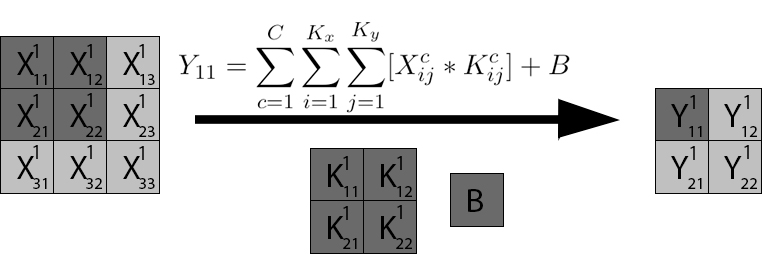
\includegraphics[width=0.8\linewidth]{imagenes/conv_ejemplo_backprop_1.jpg} 
	\caption{Ejemplo de propagación hacia delante en una capa convolucional}
	\label{fig:ejemplo_forward_prop_convolucional}
\end{figure}

La figura \ref{fig:ejemplo_forward_prop_convolucional} ilustra el ejemplo de propagación hacia delante que se utilizará en esta sección. En dicha figura, \textit{C} representa el número de canales de profundidad del volumen de entrada \textit{X}, mientras que ${K_x}$ y ${K_y}$ se refieren al número de filas y columnas del kernel \textit{K} utilizado, respectivamente. \\
Siguiendo la notación empleada en secciones anteriores, se denotará por $A^c_{ij}$ al valor de $X^c_{ij}$ antes de aplicar la función de activación correspondiente, y por $Z^c_{ij}$ al valor resultante después de aplicar dicha función.

\subsubsection{Sumatoria de gradientes}

\begin{gather}
	\frac{\partial E}{\partial K^c_{11}} = \sum_{i=1}^{I}\sum_{j=1}^{J}  [\frac{\partial E}{\partial Y^c_{ij}} * \frac{\partial Y^c_{ij}}{\partial K^c_{11}}] \\
	\frac{\partial E}{\partial X^c_{11}} = \sum_{i=1}^{I}\sum_{j=1}^{J}  [\frac{\partial E}{\partial Y^c_{ij}} * \frac{\partial Y^c_{ij}}{\partial Z^c_{11}} * \frac{\partial Z^c_{ij}}{\partial A^c_{11}}] 
\end{gather}

Para calcular el gradiente de la función de error con respecto a cada peso ${K_{xy}}$ o entrada ${X_{xy}}$, se debe realizar una sumatoria del gradiente correspondiente sobre cada valor de salida producido por la convolución. En el caso de los pesos asociados a un canal de profundidad $c \in C$, cada peso ${K_{xy}}$ se empleó en el cálculo de cada valor $Y^c_{ij}$. Por otro lado, los valores de la entrada ${X_{xy}}$ contribuyen al cálculo de varios valores de salida $\{Y_1, Y_2\} \in Y$. Este proceso fue detallado anteriormente en la sección \ref{intro_CNN}.

\subsubsection{Gradiente de $Y^c_{11}$}

\begin{gather}
	Y^c_{11} = Z^c_{11} * K^c_{11} + Z^c_{12} * K^c_{12} + Z^c_{21} * K^c_{21} + Z^c_{22} * K^c_{22} \label{grad_y11_k_11} \\
	\frac{\partial Y^c_{11}}{\partial K^c_{xy}} = \frac{\partial (Z^c_{11} * K^c_{11} + Z^c_{12} * K^c_{12} + Z^c_{21} * K^c_{21} + Z^c_{22} * K^c_{22})}{\partial K^c_{xy}} \label{grad_y11_k_12} \\
	\frac{\partial Y^c_{11}}{\partial K^c_{11}} = Z^c_{11}, \hspace{10mm} \frac{\partial Y^c_{11}}{\partial K^c_{12}} = Z^c_{12} \label{grad_y11_k_21}\\
	\frac{\partial Y^c_{11}}{\partial K^c_{21}} = Z^c_{21}, \hspace{10mm} \frac{\partial Y^c_{11}}{\partial K^c_{22}} = Z^c_{22} \label{grad_y11_k_22}
\end{gather}

\begin{gather}
	\frac{\partial Y^c_{11}}{\partial Z^c_{11}} = K^c_{11}, \hspace{10mm} \frac{\partial Y^c_{11}}{\partial Z^c_{12}} = K^c_{12}, \hspace{10mm} \frac{\partial Y^c_{11}}{\partial Z^c_{13}} = 0 \label{grad_y11_z_1} \\
	\frac{\partial Y^c_{11}}{\partial Z^c_{21}} = K^c_{21}, \hspace{10mm} \frac{\partial Y^c_{11}}{\partial Z^c_{22}} = K^c_{22}, \hspace{10mm} \frac{\partial Y^c_{11}}{\partial Z^c_{23}} = 0 \label{grad_y11_z_2} \\
	\frac{\partial Y^c_{11}}{\partial Z^c_{31}} = 0, \hspace{15mm} \frac{\partial Y^c_{11}}{\partial Z^c_{32}} = 0, \hspace{15mm} \frac{\partial Y^c_{11}}{\partial Z^c_{33}} = 0 \label{grad_y11_z_3}
\end{gather}

La fórmula \ref{grad_y11_k_11}, presenta una descomposición de $Y^c_{11}$ en términos de $Z$ y $K$. Esto, es esencial para el cálculo del gradiente, tanto con respecto a Z, (como se detalla en las fórmulas \ref{grad_y11_z_1}, \ref{grad_y11_z_2}, \ref{grad_y11_z_3}), como con respecto a K, (como se muestra en las fórmulas \ref{grad_y11_k_12}, \ref{grad_y11_k_21}, \ref{grad_y11_k_22}). Esta descomposición, permite calcular el gradiente de $Y^c_{11}$ con respecto a cada parámetro de la capa convolucional. \\
Cabe destacar que, para calcular el gradiente con respecto a cada valor del volumen de entrada (X), también debe calcularse la derivada de la función de activación asociada a dicha capa. Es decir, $\frac{\partial Z}{\partial A}$. Sin embargo, dado que este proceso ha sido abordado en secciones anteriores, se omitirá en esta ocasión, al igual que el cálculo del gradiente con respecto al sesgo de cada capa. El propósito de esta omisión es evitar cálculos redundantes y concentrar la atención en los aspectos más relevantes e innovadores. No obstante, es importante señalar que todos los cálculos discutidos en esta documentación, y más, están implementados en el código correspondiente, lo que garantiza que este conocimiento se ha aplicado y verificado en la práctica. \\
Además, dado que todo ha sido realizado manualmente por la misma persona, la mayoría de las variables e índices utilizados en la documentación coinciden perfectamente o son muy similares a los empleados en el código. Esto asegura que cualquier lector con conocimientos básicos de programación pueda comprender gran parte de las implementaciones desarrolladas en este proyecto.

\subsubsection{Gradiente de $Y^c_{12}$}

\begin{figure}[H]
	\centering
	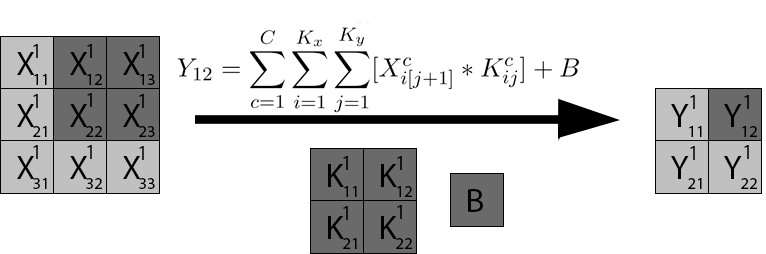
\includegraphics[width=1\linewidth]{imagenes/conv_ejemplo_backprop_2.jpg} 
	\caption{Cálculo de $Y^c_{12}$ mediante propagación hacia delante en una capa convolucional}
	\label{fig:ejemplo_2_forward_prop_convolucional}
\end{figure}

Del mismo modo, se calcula el gradiente de $Y^c_{12}$ con respecto a cada peso, como se muestra en las fórmulas \ref{grad_y12_k_1} y \ref{grad_y12_k_2}.

\begin{gather}
	Y^c_{12} = Z^c_{12} * K^c_{11} + Z^c_{13} * K^c_{12} + Z^c_{22} * K^c_{21} + Z^c_{23} * K^c_{22} \\
	\frac{\partial Y^c_{12}}{\partial K^c_{xy}} = \frac{\partial (Z^c_{11} * K^c_{11} + Z^c_{12} * K^c_{12} + Z^c_{21} * K^c_{21} + Z^c_{22} * K^c_{22})}{\partial K^c_{xy}} \\
	\frac{\partial Y^c_{12}}{\partial K^c_{11}} = Z^c_{12}, \hspace{10mm} \frac{\partial Y^c_{12}}{\partial K^c_{12}} = Z^c_{13} \label{grad_y12_k_1} \\
	\frac{\partial Y^c_{12}}{\partial K^c_{21}} = Z^c_{22}, \hspace{10mm} \frac{\partial Y^c_{12}}{\partial K^c_{22}} = Z^c_{23} \label{grad_y12_k_2}
\end{gather}

Asimismo, se calcula el gradiente de $Y^c_{12}$ con respecto a cada valor de entrada, como se detalla en las fórmulas \ref{grad_y12_z_1}, \ref{grad_y12_z_2} y \ref{grad_y12_z_3}.

\begin{gather}
	\frac{\partial Y^c_{12}}{\partial Z^c_{11}} = 0, \hspace{10mm} \frac{\partial Y^c_{12}}{\partial Z^c_{12}} = K^c_{11}, \hspace{10mm} \frac{\partial Y^c_{12}}{\partial Z^c_{13}} = K^c_{12} \label{grad_y12_z_1} \\
	\frac{\partial Y^c_{12}}{\partial Z^c_{21}} = 0, \hspace{10mm} \frac{\partial Y^c_{12}}{\partial Z^c_{22}} = K^c_{21}, \hspace{10mm} \frac{\partial Y^c_{12}}{\partial Z^c_{23}} = K^c_{22} \label{grad_y12_z_2} \\
	\frac{\partial Y^c_{12}}{\partial Z^c_{31}} = 0, \hspace{10mm} \frac{\partial Y^c_{12}}{\partial Z^c_{32}} = 0, \hspace{15mm} \frac{\partial Y^c_{12}}{\partial Z^c_{33}} = 0 \hspace{5mm} \label{grad_y12_z_3}
\end{gather}

\subsubsection{Gradiente de $Y^c_{21}$}

\begin{figure}[H]
	\centering
	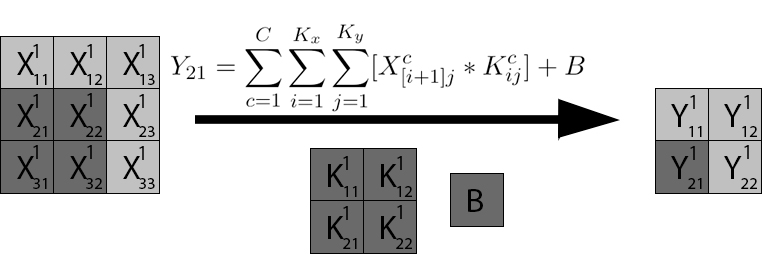
\includegraphics[width=1\linewidth]{imagenes/conv_ejemplo_backprop_3.jpg} 
	\caption{Cálculo de $Y^c_{21}$ mediante propagación hacia delante en una capa convolucional}
	\label{fig:ejemplo_3_forward_prop_convolucional}
\end{figure}

Se calcula el gradiente de $Y^c_{21}$ con respecto a cada peso, tal y como se muestra en las ecuaciones \ref{grad_y21_k_1} y \ref{grad_y21_k_2}.

\begin{gather}
	Y^c_{21} = Z^c_{21} * K^c_{11} + Z^c_{22} * K^c_{12} + Z^c_{31} * K^c_{21} + Z^c_{32} * K^c_{22} \\
	\frac{\partial Y^c_{21}}{\partial K^c_{xy}} = \frac{\partial (Z^c_{21} * K^c_{11} + Z^c_{22} * K^c_{12} + Z^c_{31} * K^c_{21} + Z^c_{32} * K^c_{22})}{\partial K^c_{xy}} \\
	\frac{\partial Y^c_{21}}{\partial K^c_{11}} = Z^c_{21}, \hspace{10mm} \frac{\partial Y^c_{21}}{\partial K^c_{12}} = Z^c_{22} \label{grad_y21_k_1} \\
	\frac{\partial Y^c_{21}}{\partial K^c_{21}} = Z^c_{31}, \hspace{10mm} \frac{\partial Y^c_{21}}{\partial K^c_{22}} = Z^c_{32} \label{grad_y21_k_2}
\end{gather}

Asimismo, se calcula el gradiente de $Y^c_{21}$ con respecto a cada valor de entrada, según se detalla en las ecuaciones \ref{grad_y21_z_1}, \ref{grad_y21_z_2} y \ref{grad_y21_z_3}.
 
\begin{gather}
	\frac{\partial Y^c_{21}}{\partial Z^c_{11}} = 0, \hspace{16mm} \frac{\partial Y^c_{21}}{\partial Z^c_{12}} = 0, \hspace{13mm} \frac{\partial Y^c_{21}}{\partial Z^c_{13}} = 0 \label{grad_y21_z_1} \\
	\frac{\partial Y^c_{21}}{\partial Z^c_{21}} = K^c_{11}, \hspace{10mm} \frac{\partial Y^c_{21}}{\partial Z^c_{22}} = K^c_{12}, \hspace{10mm} \frac{\partial Y^c_{21}}{\partial Z^c_{23}} = 0 \label{grad_y21_z_2} \\
	\frac{\partial Y^c_{21}}{\partial Z^c_{31}} = K^c_{21}, \hspace{10mm} \frac{\partial Y^c_{21}}{\partial Z^c_{32}} = K^c_{22}, \hspace{10mm} \frac{\partial Y^c_{21}}{\partial Z^c_{33}} = 0 \label{grad_y21_z_3}
\end{gather}


\subsubsection{Gradiente de $Y^c_{22}$}

\begin{figure}[H]
	\centering
	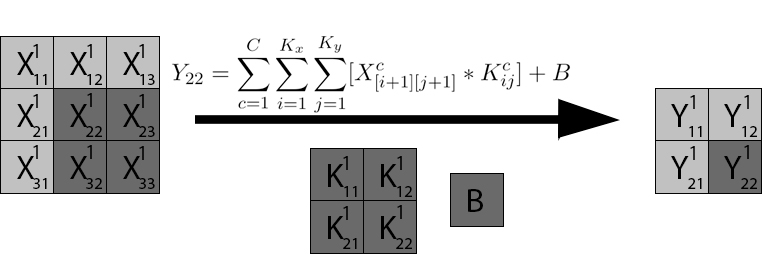
\includegraphics[width=1\linewidth]{imagenes/conv_ejemplo_backprop_4.jpg} 
	\caption{Cálculo de $Y^c_{22}$ mediante propagación hacia delante en una capa convolucional}
	\label{fig:ejemplo_4_forward_prop_convolucional}
\end{figure}

El gradiente de $Y^c_{22}$ se calcula con respecto a cada peso, como se muestra en las fórmulas \ref{grad_y22_k_1} y \ref{grad_y22_k_2}.

\begin{gather}
	Y^c_{22} = Z^c_{22} * K^c_{11} + Z^c_{23} * K^c_{12} + Z^c_{32} * K^c_{21} + Z^c_{33} * K^c_{22} \\
	\frac{\partial Y^c_{22}}{\partial K^c_{xy}} = \frac{\partial (Z^c_{11} * K^c_{11} + Z^c_{12} * K^c_{12} + Z^c_{21} * K^c_{21} + Z^c_{22} * K^c_{22})}{\partial K^c_{xy}} \\
	\frac{\partial Y^c_{22}}{\partial K^c_{11}} = Z^c_{22}, \hspace{10mm} \frac{\partial Y^c_{22}}{\partial K^c_{12}} = Z^c_{23} \label{grad_y22_k_1} \\
	\frac{\partial Y^c_{22}}{\partial K^c_{21}} = Z^c_{32}, \hspace{10mm} \frac{\partial Y^c_{22}}{\partial K^c_{22}} = Z^c_{33} \label{grad_y22_k_2}
\end{gather}

Se calcula el gradiente de $Y^c_{22}$ respecto a cada valor del volumen de entrada, como se muestra en las fórmulas \ref{grad_y22_z_1}, \ref{grad_y22_z_2}, y \ref{grad_y22_z_3}.

\begin{gather}
	\frac{\partial Y^c_{22}}{\partial Z^c_{11}} = 0, \hspace{10mm} \frac{\partial Y^c_{22}}{\partial Z^c_{12}} = 0, \hspace{15mm} \frac{\partial Y^c_{22}}{\partial Z^c_{13}} = 0 \hspace{4mm} \label{grad_y22_z_1} \\
	\frac{\partial Y^c_{22}}{\partial Z^c_{21}} = 0, \hspace{10mm} \frac{\partial Y^c_{22}}{\partial Z^c_{22}} = K^c_{11}, \hspace{10mm} \frac{\partial Y^c_{22}}{\partial Z^c_{23}} = K^c_{12} \label{grad_y22_z_2} \\
	\frac{\partial Y^c_{22}}{\partial Z^c_{31}} = 0, \hspace{10mm} \frac{\partial Y^c_{22}}{\partial Z^c_{32}} = K^c_{21}, \hspace{10mm} \frac{\partial Y^c_{22}}{\partial Z^c_{33}} = K^c_{22} \label{grad_y22_z_3}
\end{gather}

\subsubsection{Gradiente respecto a pesos como convolución}

Finalmente, se procede al cálculo de la suma total de gradientes con respecto a cada peso de la capa, conforme a las fórmulas \ref{grad_Y_K_1}, \ref{grad_Y_K_2}, \ref{grad_Y_K_3}, y \ref{grad_Y_K_4}. Se observa un patrón claro en los gradientes resultantes, que refleja la contribución de cada peso en el cálculo del error total.

\begin{gather}
	\frac{\partial E}{\partial K^c_{11}} = \frac{\partial E}{\partial Y^c_{11}} * Z^c_{11} + \frac{\partial E}{\partial Y^c_{12}} * Z^c_{12} + \frac{\partial E}{\partial Y^c_{21}} * Z^c_{21} + \frac{\partial E}{\partial Y^c_{22}} * Z^c_{22} \label{grad_Y_K_1} \\
	\frac{\partial E}{\partial K^c_{12}} = \frac{\partial E}{\partial Y^c_{11}} * Z^c_{12} + \frac{\partial E}{\partial Y^c_{12}} * Z^c_{13} + \frac{\partial E}{\partial Y^c_{21}} * Z^c_{22} + \frac{\partial E}{\partial Y^c_{22}} * Z^c_{23} \label{grad_Y_K_2} \\	
	\frac{\partial E}{\partial K^c_{21}} = \frac{\partial E}{\partial Y^c_{11}} * Z^c_{21} + \frac{\partial E}{\partial Y^c_{12}} * Z^c_{22} + \frac{\partial E}{\partial Y^c_{31}} * Z^c_{21} + \frac{\partial E}{\partial Y^c_{22}} * Z^c_{32} \label{grad_Y_K_3} \\
	\frac{\partial E}{\partial K^c_{22}} = \frac{\partial E}{\partial Y^c_{11}} * Z^c_{22} + \frac{\partial E}{\partial Y^c_{12}} * Z^c_{23} + \frac{\partial E}{\partial Y^c_{31}} * Z^c_{32} + \frac{\partial E}{\partial Y^c_{22}} * Z^c_{33} \label{grad_Y_K_4}
\end{gather}

Como se observa en los cálculos realizados, estos coinciden con una operación de convolución entre la entrada \textit{X} y el gradiente respecto a la capa de salida \textit{Y}. Este procedimiento se detalla en la Figura \ref{fig:conv_backprop_como_convolucion_X_Y} \cite{conv_backprop}.

\begin{figure}[H]
	\centering
	\begin{subfigure}{.5\textwidth}
		\hspace{-25mm}
		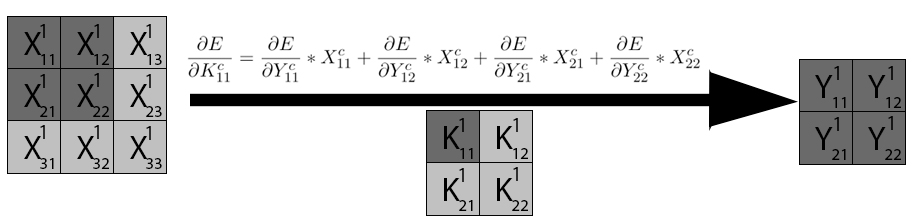
\includegraphics[width=1.4\linewidth]{imagenes/conv_backprop_1.jpg}  
		\caption{Cálculo de $\frac{\partial E}{\partial K^1_{11}}$}
	\end{subfigure}%
	\begin{subfigure}{.5\textwidth}
		\hspace{5mm}
		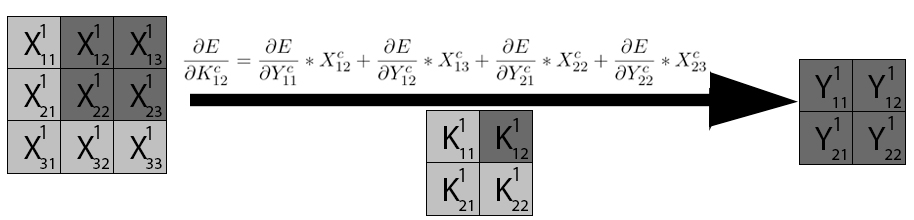
\includegraphics[width=1.4\linewidth]{imagenes/conv_backprop_2.jpg}  
		\caption{Cálculo de $\frac{\partial E}{\partial K^1_{12}}$}
	\end{subfigure}
	\vspace{5mm}
	\begin{subfigure}{.5\textwidth}
	\hspace{-25mm}
	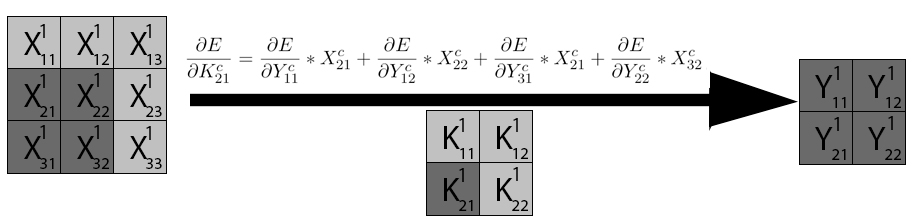
\includegraphics[width=1.4\linewidth]{imagenes/conv_backprop_3.jpg}  
	\caption{Cálculo de $\frac{\partial E}{\partial K^1_{21}}$}
	\end{subfigure}%
	\begin{subfigure}{.5\textwidth}
	\hspace{5mm}
	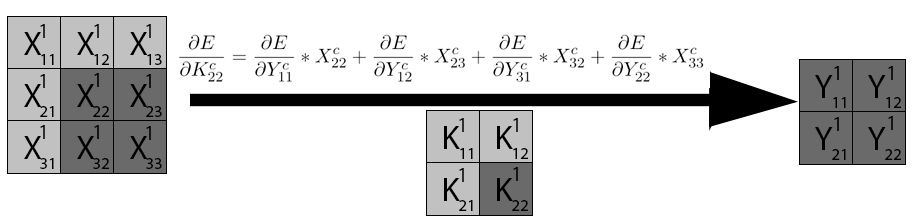
\includegraphics[width=1.4\linewidth]{imagenes/conv_backprop_4.jpg}  
	\caption{Cálculo de $\frac{\partial E}{\partial K^1_{22}}$}
	\end{subfigure}
	\caption{Cálculo del gradiente de la pérdida con respecto a cada filtro como convolución entre X e Y}
	\label{fig:conv_backprop_como_convolucion_X_Y}
\end{figure}

En la figura \ref{fig:conv_backprop_como_convolucion_X_Y}, cada subfigura $\{(a), (b), (c), (d)\}$ representa el cálculo del gradiente con respecto a un peso específico. Aunque la representación puede parecer algo diferente a simple vista, los cálculos son esencialmente los mismos que los obtenidos anteriormente, con la única diferencia en la forma en que se visualizan.

\subsubsection{Gradiente respecto a entrada como convolución}

Por razones de simplicidad, y en consonancia con las recomendaciones de expertos, y la experiencia personal, se empleará ReLU como función de activación en las capas convolucionales. Dado que, la derivada de esta función ya ha sido previamente calculada, (véase la fórmula \ref{deriv_relu}), se considerará esta información para los cálculos subsiguientes.


\begin{gather}
	\frac{\partial E}{\partial A^c_{11}} = \frac{\partial E}{\partial Y^c_{11}} * K^c_{11} *  ReLU'(A^c_{11}) \\
	\frac{\partial E}{\partial A^c_{12}} = (\frac{\partial E}{\partial Y^c_{11}} * K^c_{12} + \frac{\partial E}{\partial Y^c_{12}} * K^c_{11}) * ReLU'(A^c_{12}) \\
	\frac{\partial E}{\partial A^c_{13}} = \frac{\partial E}{\partial Y^c_{12}} * K^c_{12} * ReLU'(A^c_{13}) \\
\end{gather}

\begin{gather}
	\frac{\partial E}{\partial A^c_{21}} = (\frac{\partial E}{\partial Y^c_{11}} * K^c_{21} + \frac{\partial E}{\partial Y^c_{21}} * K^c_{11}) * ReLU'(A^c_{21}) \\
	\frac{\partial E}{\partial A^c_{22}} = (\frac{\partial E}{\partial Y^c_{11}} * K^c_{22} + \frac{\partial E}{\partial Y^c_{12}} * K^c_{21} + \frac{\partial E}{\partial Y^c_{21}} * K^c_{12} + \frac{\partial E}{\partial Y^c_{22}} * K^c_{11}) * ReLU'(A^c_{22}) \\
	\frac{\partial E}{\partial A^c_{23}} = (\frac{\partial E}{\partial Y^c_{12}} * K^c_{22} + \frac{\partial E}{\partial Y^c_{22}} * K^c_{12}) * ReLU'(A^c_{22})\\
\end{gather}

\begin{gather}
	\frac{\partial E}{\partial A^c_{31}} = \frac{\partial E}{\partial Y^c_{21}} * K^c_{21} * ReLU'(A^c_{31})\\
	\frac{\partial E}{\partial A^c_{32}} = (\frac{\partial E}{\partial Y^c_{21}} * K^c_{22} + \frac{\partial E}{\partial Y^c_{22}} * K^c_{21}) * ReLU'(A^c_{32})\\
	\frac{\partial E}{\partial A^c_{33}} = \frac{\partial E}{\partial Y^c_{22}} * K^c_{22} * ReLU'(A^c_{33})
\end{gather}

Tal y como se observa en los cálculos obtenidos, estos corresponden a una convolución de tipo ``full'' (completa) entre el gradiente con respecto a la capa de salida (Y) y los pesos (K), invertidos tanto horizontal como verticalmente. El proceso de cálculo del gradiente con respecto a cada valor $x \in X$ se presenta en detalle en la figura \ref{fig:conv_backprop_como_convolucion_Y_W}, mientras que la manera de invertir los pesos se ilustra en la figura \ref{fig:flip_W} \cite{conv_backprop}.

\begin{figure}[H]
	\centering
	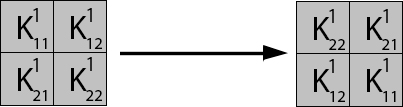
\includegraphics[width=0.8\linewidth]{imagenes/flip_pesos.jpg}  
	\caption{Inversión de los pesos en K tanto horizontal como verticalmente}
	\label{fig:flip_W}
\end{figure}

\begin{figure}[H]
	\centering
	\begin{subfigure}{.5\textwidth}
		\hspace{-25mm}
		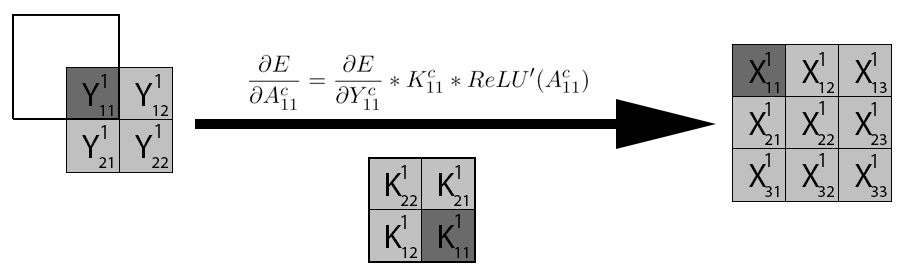
\includegraphics[width=1.4\linewidth]{imagenes/conv_back_entrada_1.jpg}  
		\caption{Gradiente con respecto a $X^1_{11}$}
	\end{subfigure}%
	\begin{subfigure}{.5\textwidth}
		\hspace{5mm}
		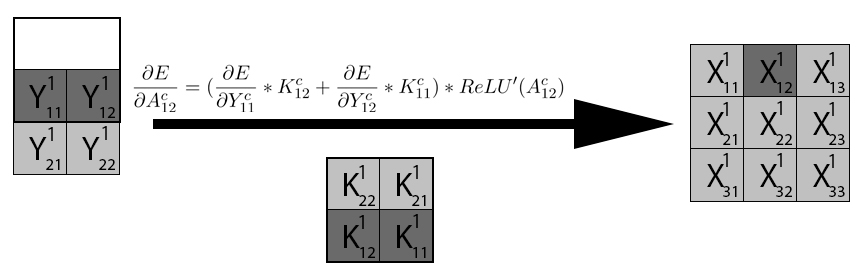
\includegraphics[width=1.4\linewidth]{imagenes/conv_back_entrada_2.jpg}  
		\caption{Gradiente con respecto a $X^1_{12}$}
	\end{subfigure}
	\vspace{5mm}
	\begin{subfigure}{.5\textwidth}
		\hspace{-25mm}
		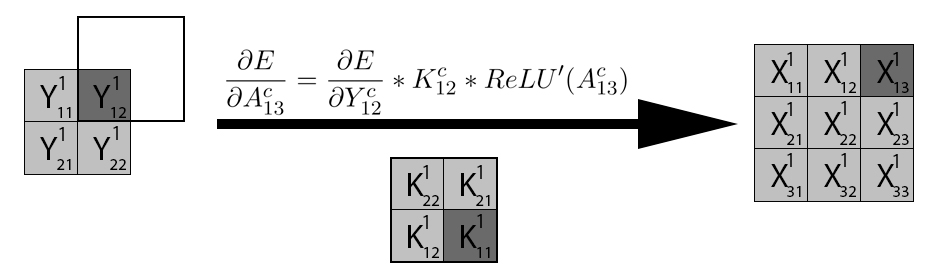
\includegraphics[width=1.4\linewidth]{imagenes/conv_back_entrada_3.jpg}  
		\caption{Gradiente con respecto a $X^1_{13}$}
	\end{subfigure}%
	\begin{subfigure}{.5\textwidth}
		\hspace{5mm}
		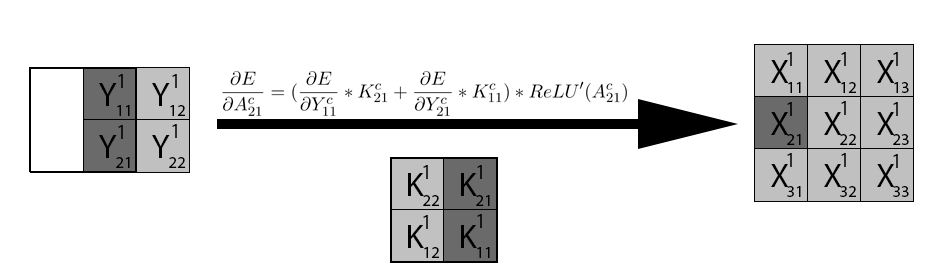
\includegraphics[width=1.4\linewidth]{imagenes/conv_back_entrada_4.jpg}  
		\caption{Gradiente con respecto a $X^1_{21}$}
	\end{subfigure}
		\vspace{5mm}
	\begin{subfigure}{.5\textwidth}
		\hspace{-25mm}
		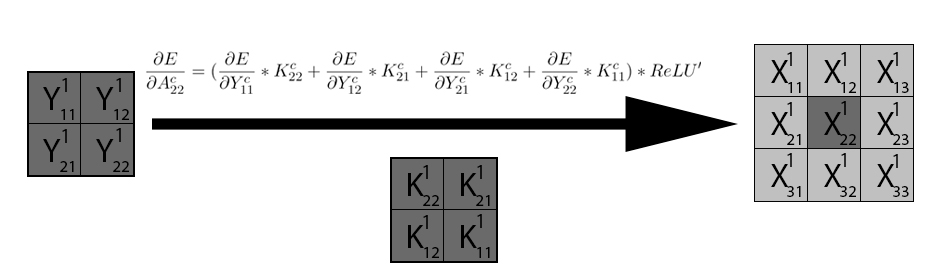
\includegraphics[width=1.4\linewidth]{imagenes/conv_back_entrada_5.jpg}  
		\caption{Gradiente con respecto a $X^1_{22}$}
	\end{subfigure}%
	\begin{subfigure}{.5\textwidth}
		\hspace{5mm}
		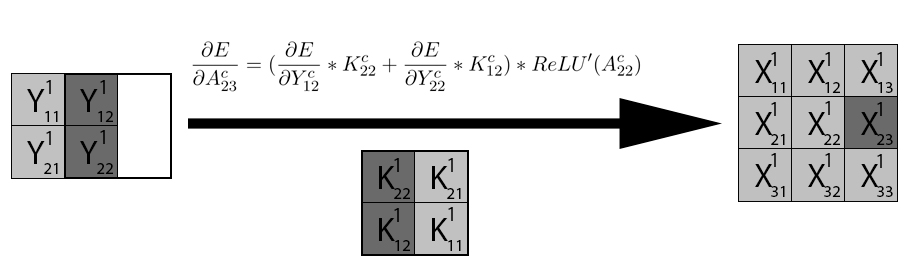
\includegraphics[width=1.4\linewidth]{imagenes/conv_back_entrada_6.jpg}  
		\caption{Gradiente con respecto a $X^1_{23}$}
	\end{subfigure}
		\vspace{5mm}
	\begin{subfigure}{.5\textwidth}
		\hspace{-25mm}
		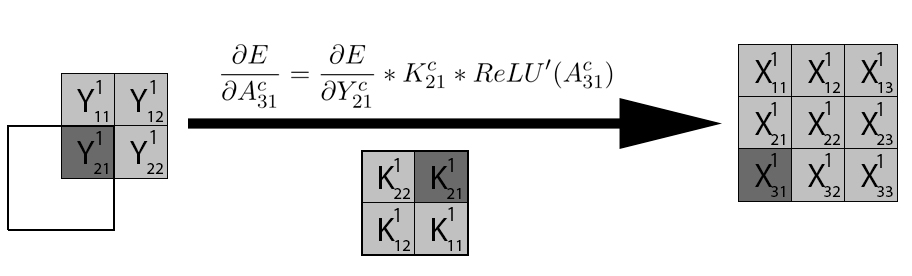
\includegraphics[width=1.4\linewidth]{imagenes/conv_back_entrada_7.jpg}  
		\caption{Gradiente con respecto a $X^1_{31}$}
	\end{subfigure}%
	\begin{subfigure}{.5\textwidth}
		\hspace{5mm}
		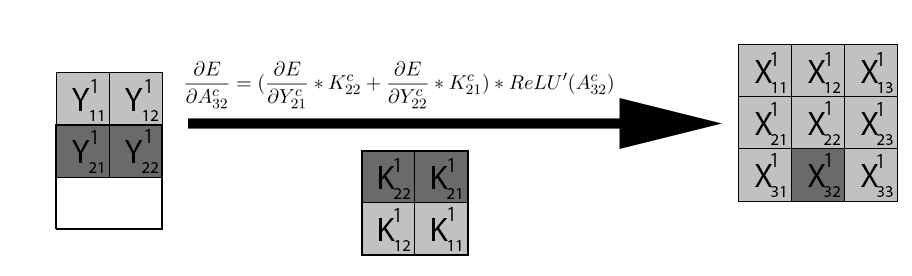
\includegraphics[width=1.4\linewidth]{imagenes/conv_back_entrada_8.jpg}  
		\caption{Gradiente con respecto a $X^1_{32}$}
	\end{subfigure}
		\vspace{5mm}
	\begin{subfigure}{.5\textwidth}
		\hspace{-25mm}
		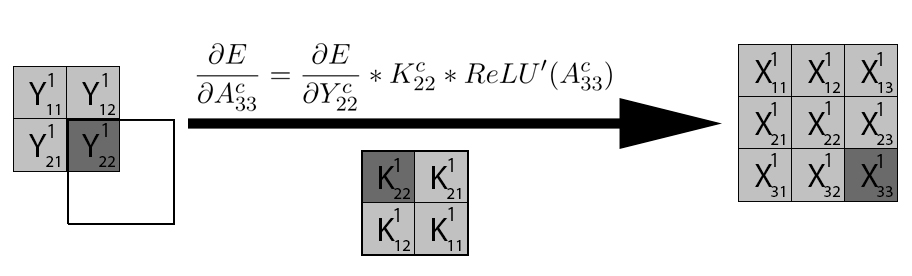
\includegraphics[width=1.4\linewidth]{imagenes/conv_back_entrada_9.jpg}  
		\caption{Gradiente con respecto a $X^1_{33}$}
	\end{subfigure}
	\caption{Cálculo del gradiente de la pérdida con respecto a cada valor de entrada como convolución entre K e Y}
	\label{fig:conv_backprop_como_convolucion_Y_W}
\end{figure}

Una vez más, los cálculos presentados en la Figura \ref{fig:conv_backprop_como_convolucion_Y_W} coinciden perfectamente con los obtenidos anteriormente, ya que son idénticos. La única diferencia radica en la manera de presentación, la cual ha sido adaptada para ofrecer una comprensión más y generalizada del proceso. Esta adaptación facilita la automatización de los cálculos y permite una implementación más eficiente en el código.

\subsection{Retropropagación con relleno}

\begin{figure}[H]
	\centering
	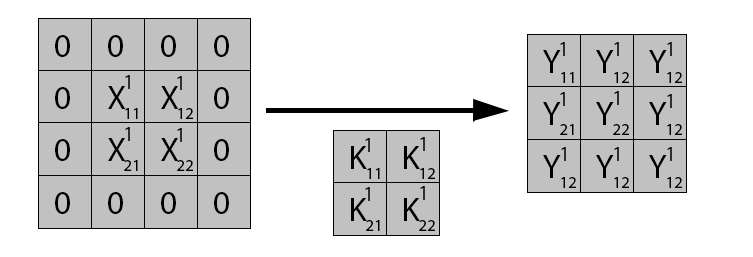
\includegraphics[width=0.8\linewidth]{imagenes/conv_back_padding_intro.jpg} 
	\caption{Ejemplo de retropropagación en una capa convolucional con relleno}
	\label{fig:conv_back_padding_intro}
\end{figure}

De manera similar al apartado anterior, se realizará y presentará el cálculo de la retropropagación para una capa convolucional. La diferencia principal en este caso radica en la inclusión de relleno en la capa, como se ilustra en el ejemplo proporcionado en la Figura \ref{fig:conv_back_padding_intro}. En consecuencia, se procederá a calcular el gradiente de la función de error con respecto a los pesos y a los valores de entrada de la capa.

\subsubsection{Gradiente de $Y^c_{11}$}

\begin{figure}[H]
	\centering
	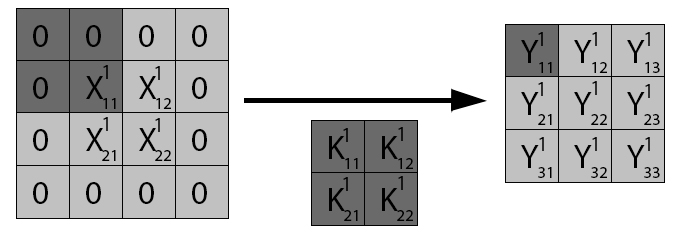
\includegraphics[width=0.8\linewidth]{imagenes/conv_back_padding_1.jpg} 
	\caption{Retropropagación de $Y^c_{11}$}
\end{figure}

Para facilitar la compresión del lector, se conservará la misma estructura y notación empleadas en el apartado anterior. Así, se procederá al cálculo del gradiente de $Y^c_{11}$ con respecto a cada peso utilizando las fórmulas \ref{gradr_Y11_w_1} y \ref{gradr_Y11_w_1}.

\begin{gather}
	Y^c_{11} = Z^c_{11} * K^c_{22} \\
	\frac{\partial Y^c_{11}}{\partial K^c_{xy}} = \frac{\partial (Z^c_{11} * K^c_{22})}{\partial K^c_{xy}} \\
	\frac{\partial Y^c_{11}}{\partial K^c_{11}} = 0, \hspace{10mm} \frac{\partial Y^c_{11}}{\partial K^c_{12}} = 0 \hspace{3mm} \label{gradr_Y11_w_1} \\
	\frac{\partial Y^c_{11}}{\partial K^c_{21}} = 0, \hspace{10mm} \frac{\partial Y^c_{11}}{\partial K^c_{22}} = Z^c_{11} \label{gradr_Y11_w_2}
\end{gather}

Para mantener la coherencia con el apartado anterior, también se calculará el gradiente de $Y^c_{11}$ con respecto a cada valor del volumen de entrada utilizando las fórmulas \ref{gradr_Y11_z_1} y \ref{gradr_Y11_z_2}.

\begin{gather}
	\frac{\partial Y^c_{11}}{\partial Z^c_{11}} = K^c_{22}, \hspace{10mm} \frac{\partial Y^c_{11}}{\partial Z^c_{12}} = 0 \label{gradr_Y11_z_1} \\
	\frac{\partial Y^c_{11}}{\partial Z^c_{21}} = 0, \hspace{14mm} \frac{\partial Y^c_{11}}{\partial Z^c_{22}} = 0 \label{gradr_Y11_z_2}
\end{gather}


\subsubsection{Gradiente de $Y^c_{12}$}

\begin{figure}[H]
	\centering
	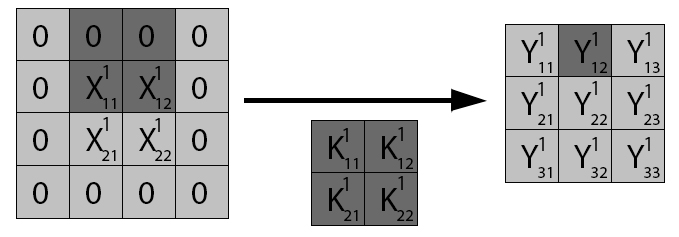
\includegraphics[width=0.8\linewidth]{imagenes/conv_back_padding_2.jpg} 
	\caption{Retropropagación de $Y^c_{12}$}
\end{figure}

Se calculará el gradiente de $Y^c_{12}$ con respecto a cada peso utilizando las fórmulas \ref{gradr_Y12_w_1} y \ref{gradr_Y12_w_2}.

\begin{gather}
	Y^c_{12} = Z^c_{11} * K^c_{21} + Z^c_{12} * K^c_{22} \\
	\frac{\partial Y^c_{12}}{\partial K^c_{xy}} = \frac{\partial (Z^c_{11} * K^c_{21} + Z^c_{12} * K^c_{22})}{\partial K^c_{xy}} \\
	\frac{\partial Y^c_{12}}{\partial K^c_{11}} = 0, \hspace{10mm} \frac{\partial Y^c_{12}}{\partial K^c_{12}} = 0 \label{gradr_Y12_w_1} \\
	\frac{\partial Y^c_{12}}{\partial K^c_{21}} = Z^c_{11}, \hspace{10mm} \frac{\partial Y^c_{12}}{\partial K^c_{22}} = Z^c_{12} \label{gradr_Y12_w_2}
\end{gather}

Asimismo, se calculará el gradiente de $Y^c_{12}$ con respecto a cada valor del volumen de entrada utilizando las fórmulas \ref{gradr_Y12_z_1} y \ref{gradr_Y12_z_2}.

\begin{gather}
	\frac{\partial Y^c_{12}}{\partial Z^c_{11}} = K^c_{21}, \hspace{10mm} \frac{\partial Y^c_{12}}{\partial Z^c_{12}} = K^c_{22} \label{gradr_Y12_z_1} \\
	\frac{\partial Y^c_{12}}{\partial Z^c_{21}} = 0, \hspace{14mm} \frac{\partial Y^c_{12}}{\partial Z^c_{22}} = 0 \hspace{4mm} \label{gradr_Y12_z_2}
\end{gather}

\subsubsection{Gradiente de $Y^c_{13}$}

\begin{figure}[H]
	\centering
	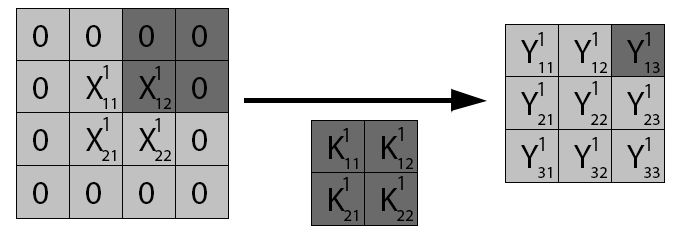
\includegraphics[width=0.8\linewidth]{imagenes/conv_back_padding_3.jpg} 
	\caption{Retropropagación de $Y^c_{13}$}
\end{figure}

Se calculará el gradiente de $Y^c_{13}$ con respecto a cada peso mediante las fórmulas \ref{gradr_Y13_w_1} y \ref{gradr_Y13_w_2}.

\begin{gather}
	Y^c_{13} = Z^c_{12} * K^c_{21} \\
	\frac{\partial Y^c_{13}}{\partial K^c_{xy}} = \frac{\partial (Z^c_{12} * K^c_{21})}{\partial K^c_{xy}} \\
	\frac{\partial Y^c_{13}}{\partial K^c_{11}} = 0, \hspace{13mm} \frac{\partial Y^c_{13}}{\partial K^c_{12}} = 0 \label{gradr_Y13_w_1} \\
	\frac{\partial Y^c_{13}}{\partial K^c_{21}} = Z^c_{12}, \hspace{10mm} \frac{\partial Y^c_{13}}{\partial K^c_{22}} = 0
\end{gather} \label{gradr_Y13_w_2}

Además, se calculará el gradiente de $Y^c_{13}$ con respecto a cada valor del volumen de entrada mediante las fórmulas \ref{gradr_Y13_z_1} y \ref{gradr_Y13_z_2}.

\begin{gather}
	\frac{\partial Y^c_{13}}{\partial Z^c_{11}} = 0, \hspace{10mm} \frac{\partial Y^c_{13}}{\partial Z^c_{12}} = K^c_{21} \label{gradr_Y13_z_1} \\
	\frac{\partial Y^c_{13}}{\partial Z^c_{21}} = 0, \hspace{14mm} \frac{\partial Y^c_{13}}{\partial Z^c_{22}} = 0 \hspace{4mm} \label{gradr_Y13_z_2}
\end{gather}


\subsubsection{Gradiente de $Y^c_{21}$}

\begin{figure}[H]
	\centering
	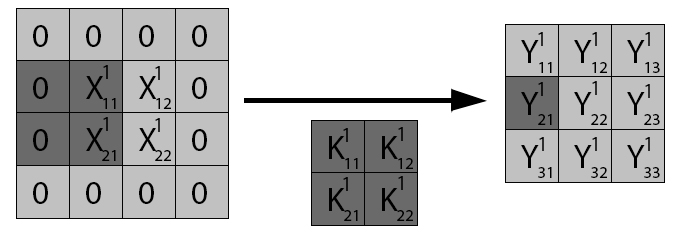
\includegraphics[width=0.8\linewidth]{imagenes/conv_back_padding_4.jpg} 
	\caption{Retropropagación de $Y^c_{21}$}
\end{figure}

Se calculará el gradiente de $Y^c_{21}$ con respecto a cada peso utilizando las fórmulas \ref{gradr_Y21_w_1} y \ref{gradr_Y21_w_2}.


\begin{gather}
	Y^c_{21} = Z^c_{11} * K^c_{12} + Z^c_{21} * K^c_{22} \\
	\frac{\partial Y^c_{21}}{\partial K^c_{xy}} = \frac{\partial (Z^c_{11} * K^c_{12} + Z^c_{21} * K^c_{22})}{\partial K^c_{xy}} \\
	\frac{\partial Y^c_{21}}{\partial K^c_{11}} = 0, \hspace{10mm} \frac{\partial Y^c_{21}}{\partial K^c_{12}} = Z^c_{11} \label{gradr_Y21_w_1} \\
	\frac{\partial Y^c_{21}}{\partial K^c_{21}} = 0, \hspace{10mm} \frac{\partial Y^c_{21}}{\partial K^c_{22}} = Z^c_{21} \label{gradr_Y21_w_2}
\end{gather}

Además, se calculará el gradiente de $Y^c_{21}$ con respecto a cada valor del volumen de entrada utilizando las fórmulas \ref{gradr_Y21_z_1} y \ref{gradr_Y21_z_2}.

\begin{gather}
	\frac{\partial Y^c_{21}}{\partial Z^c_{11}} = K^c_{12}, \hspace{10mm} \frac{\partial Y^c_{21}}{\partial Z^c_{12}} = 0 \label{gradr_Y21_z_1} \\
	\frac{\partial Y^c_{21}}{\partial Z^c_{21}} = K^c_{22}, \hspace{10mm} \frac{\partial Y^c_{21}}{\partial Z^c_{22}} = 0
\end{gather} \label{gradr_Y21_z_2}

\subsubsection{Gradiente de $Y^c_{22}$}

\begin{figure}[H]
	\centering
	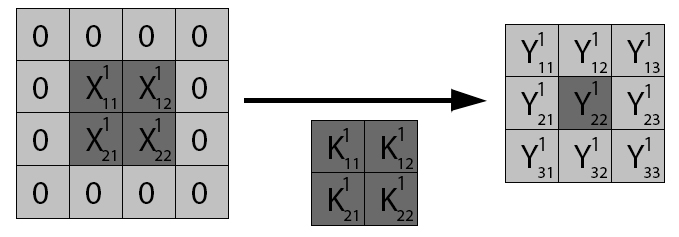
\includegraphics[width=0.8\linewidth]{imagenes/conv_back_padding_5.jpg} 
	\caption{Retropropagación de $Y^c_{22}$}
\end{figure}

Se calculará el gradiente de $Y^c_{22}$ con respecto a cada peso utilizando las fórmulas \ref{gradr_Y22_w_1} y \ref{gradr_Y22_w_2}.


\begin{gather}
	Y^c_{22} = Z^c_{11} * K^c_{11} + Z^c_{12} * K^c_{12} + Z^c_{21} * K^c_{21} + Z^c_{22} * K^c_{22} \\
	\frac{\partial Y^c_{22}}{\partial K^c_{xy}} = \frac{\partial (Z^c_{11} * K^c_{11} + Z^c_{12} * K^c_{12} + Z^c_{21} * K^c_{21} + Z^c_{22} * K^c_{22})}{\partial K^c_{xy}} \\
	\frac{\partial Y^c_{22}}{\partial K^c_{11}} = Z^c_{11}, \hspace{10mm} \frac{\partial Y^c_{22}}{\partial K^c_{12}} = Z^c_{12} \label{gradr_Y22_w_1} \\
	\frac{\partial Y^c_{22}}{\partial K^c_{21}} = Z^c_{21}, \hspace{10mm} \frac{\partial Y^c_{22}}{\partial K^c_{22}} = Z^c_{22} \label{gradr_Y22_w_2}
\end{gather}

Asimismo, se calculará el gradiente de $Y^c_{22}$ con respecto a cada valor del volumen de entrada mediante las fórmulas \ref{gradr_Y22_z_1} y \ref{gradr_Y22_z_2}.

\begin{gather}
	\frac{\partial Y^c_{22}}{\partial Z^c_{11}} = K^c_{11}, \hspace{10mm} \frac{\partial Y^c_{22}}{\partial Z^c_{12}} = K^c_{12} \label{gradr_Y22_z_1} \\
	\frac{\partial Y^c_{22}}{\partial Z^c_{21}} = K^c_{21}, \hspace{10mm} \frac{\partial Y^c_{22}}{\partial Z^c_{22}} = K^c_{22} \label{gradr_Y22_z_2}.
\end{gather}

\subsubsection{Gradiente de $Y^c_{23}$}

\begin{figure}[H]
	\centering
	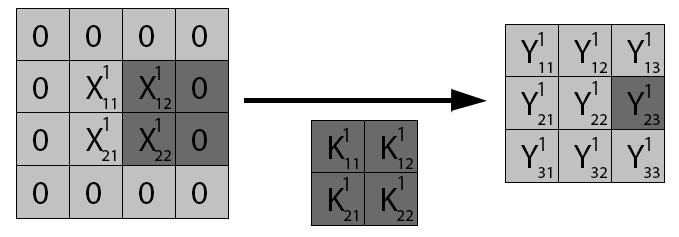
\includegraphics[width=0.8\linewidth]{imagenes/conv_back_padding_6.jpg} 
	\caption{Retropropagación de $Y^c_{23}$}
\end{figure}

Se calculará el gradiente de $Y^c_{23}$ con respecto a cada peso utilizando las fórmulas \ref{gradr_Y23_w_1} y \ref{gradr_Y23_w_2}.


\begin{gather}
	Y^c_{23} = Z^c_{12} * K^c_{11} + Z^c_{22} * K^c_{21} \\
	\frac{\partial Y^c_{23}}{\partial K^c_{xy}} = \frac{\partial (Z^c_{12} * K^c_{11} + Z^c_{22} * K^c_{21})}{\partial K^c_{xy}} \\
	\frac{\partial Y^c_{23}}{\partial K^c_{11}} = Z^c_{12}, \hspace{10mm} \frac{\partial Y^c_{23}}{\partial K^c_{12}} = 0 \label{gradr_Y23_w_1} \\
	\frac{\partial Y^c_{23}}{\partial K^c_{21}} = Z^c_{22}, \hspace{10mm} \frac{\partial Y^c_{23}}{\partial K^c_{22}} = 0 \label{gradr_Y23_w_2}
\end{gather}

De igual manera, se calculará el gradiente de $Y^c_{23}$ con respecto a cada valor del volumen de entrada mediante las fórmulas \ref{gradr_Y22_z_1} y \ref{gradr_Y22_z_2}.


\begin{gather}
	\frac{\partial Y^c_{23}}{\partial Z^c_{11}} = 0, \hspace{10mm} \frac{\partial Y^c_{23}}{\partial Z^c_{12}} = K^c_{11}\\
	\frac{\partial Y^c_{23}}{\partial Z^c_{21}} = 0, \hspace{10mm} \frac{\partial Y^c_{23}}{\partial Z^c_{22}} = K^c_{21}
\end{gather}

\subsubsection{Gradiente de $Y^c_{31}$}

\begin{figure}[H]
	\centering
	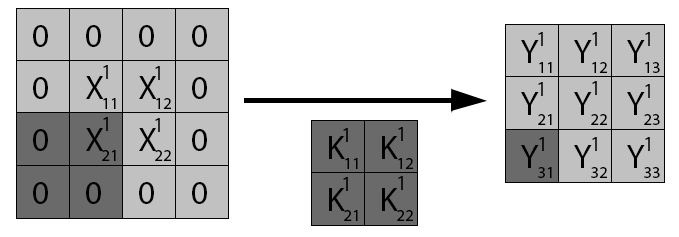
\includegraphics[width=0.8\linewidth]{imagenes/conv_back_padding_7.jpg} 
	\caption{Retropropagación de $Y^c_{31}$}
\end{figure}

Se calculará el gradiente de $Y^c_{31}$ con respecto a cada peso utilizando las fórmulas \ref{gradr_Y31_w_1} y \ref{gradr_Y31_w_2}.

\begin{gather}
	Y^c_{31} = Z^c_{21} * K^c_{12} \\
	\frac{\partial Y^c_{31}}{\partial K^c_{xy}} = \frac{\partial (Z^c_{21} * K^c_{12})}{\partial K^c_{xy}} \\
	\frac{\partial Y^c_{31}}{\partial K^c_{11}} = 0, \hspace{10mm} \frac{\partial Y^c_{31}}{\partial K^c_{12}} = Z^c_{21} \label{gradr_Y31_w_1} \\
	\frac{\partial Y^c_{31}}{\partial K^c_{21}} = 0, \hspace{10mm} \frac{\partial Y^c_{31}}{\partial K^c_{22}} = 0 \hspace{4mm} \label{gradr_Y31_w_2}
\end{gather}

Asimismo, se calculará el gradiente de $Y^c_{31}$ con respecto a cada valor del volumen de entrada mediante las fórmulas \ref{gradr_Y31_z_1} y \ref{gradr_Y31_z_2}.

\begin{gather}
	\frac{\partial Y^c_{31}}{\partial Z^c_{11}} = 0, \hspace{14mm} \frac{\partial Y^c_{31}}{\partial Z^c_{12}} = 0 \label{gradr_Y31_z_1} \\
	\frac{\partial Y^c_{31}}{\partial Z^c_{21}} = K^c_{12}, \hspace{10mm} \frac{\partial Y^c_{31}}{\partial Z^c_{22}} = 0 \label{gradr_Y31_z_2}
\end{gather}


\subsubsection{Gradiente de $Y^c_{32}$}

\begin{figure}[H]
	\centering
	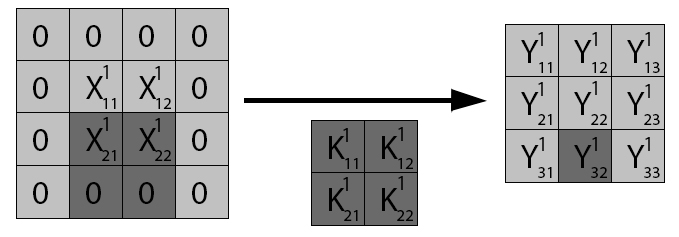
\includegraphics[width=0.8\linewidth]{imagenes/conv_back_padding_8.jpg} 
	\caption{Retropropagación de $Y^c_{32}$}
\end{figure}

Se calculará el gradiente de $Y^c_{32}$ con respecto a cada peso utilizando las fórmulas \ref{gradr_Y32_w_1} y \ref{gradr_Y32_w_2}.

\begin{gather}
	Y^c_{32} = Z^c_{21} * K^c_{11} + Z^c_{22} * K^c_{12} \\
	\frac{\partial Y^c_{32}}{\partial K^c_{xy}} = \frac{\partial (Z^c_{21} * K^c_{11} + Z^c_{22} * K^c_{12})}{\partial K^c_{xy}} \\
	\frac{\partial Y^c_{32}}{\partial K^c_{11}} = Z^c_{21}, \hspace{10mm} \frac{\partial Y^c_{32}}{\partial K^c_{12}} = Z^c_{22} \label{gradr_Y32_w_1} \\
	\frac{\partial Y^c_{32}}{\partial K^c_{21}} = 0, \hspace{14mm} \frac{\partial Y^c_{32}}{\partial K^c_{22}} = 0 \hspace{4mm} \label{gradr_Y32_w_2}
\end{gather}

Además, se calculará el gradiente de $Y^c_{32}$ con respecto a cada valor del volumen de entrada mediante las fórmulas \ref{gradr_Y32_z_1} y \ref{gradr_Y32_z_2}.


\begin{gather}
	\frac{\partial Y^c_{32}}{\partial Z^c_{11}} = 0, \hspace{14mm} \frac{\partial Y^c_{32}}{\partial Z^c_{12}} = 0 \hspace{4mm} \label{gradr_Y32_z_1} \\
	\frac{\partial Y^c_{32}}{\partial Z^c_{21}} = K^c_{11}, \hspace{10mm} \frac{\partial Y^c_{32}}{\partial Z^c_{22}} = K^c_{12} \label{gradr_Y32_z_2}
\end{gather}



\subsubsection{Gradiente de $Y^c_{33}$}

\begin{figure}[H]
	\centering
	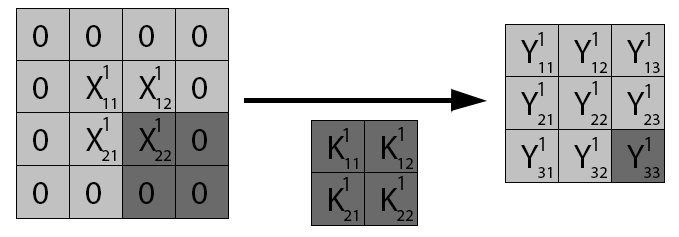
\includegraphics[width=0.8\linewidth]{imagenes/conv_back_padding_9.jpg} 
	\caption{Retropropagación de $Y^c_{33}$}
\end{figure}

Se calculará el gradiente de $Y^c_{33}$ con respecto a cada peso utilizando las fórmulas \ref{gradr_Y33_w_1} y \ref{gradr_Y33_w_2}.


\begin{gather}
	Y^c_{33} = Z^c_{22} * K^c_{11} \\
	\frac{\partial Y^c_{33}}{\partial K^c_{xy}} = \frac{\partial (Z^c_{22} * K^c_{11})}{\partial K^c_{xy}} \\
	\frac{\partial Y^c_{33}}{\partial K^c_{11}} = Z^c_{22}, \hspace{10mm} \frac{\partial Y^c_{33}}{\partial K^c_{12}} = 0 \label{gradr_Y33_w_1} \\
	\frac{\partial Y^c_{33}}{\partial K^c_{21}} = 0, \hspace{14mm} \frac{\partial Y^c_{33}}{\partial K^c_{22}} = 0 \label{gradr_Y33_w_2}
\end{gather}

Asimismo, se calculará el gradiente de $Y^c_{33}$ con respecto a cada valor del volumen de entrada utilizando las fórmulas \ref{gradr_Y33_z_1} y \ref{gradr_Y33_z_2}.


\begin{gather}
	\frac{\partial Y^c_{33}}{\partial Z^c_{11}} = 0, \hspace{10mm} \frac{\partial Y^c_{33}}{\partial Z^c_{12}} = 0 \hspace{4mm} \label{gradr_Y33_z_1} \\
	\frac{\partial Y^c_{33}}{\partial Z^c_{21}} = 0, \hspace{10mm} \frac{\partial Y^c_{33}}{\partial Z^c_{22}} = K^c_{11} \label{gradr_Y33_z_2}
\end{gather}


\subsubsection{Gradiente respecto a pesos como convolución}

Finalmente, de manera similar al caso anterior, se calcula la sumatoria de los gradientes y, con ello, el gradiente de la función de pérdida con respecto a cada peso $K_{xy}$. Nuevamente, se identifica un patrón claro en los resultados obtenidos.

\begin{gather}
	\frac{\partial E}{\partial K^c_{11}} = \frac{\partial E}{\partial Y^c_{22}} * Z^c_{11} + \frac{\partial E}{\partial Y^c_{23}} * Z^c_{12} + \frac{\partial E}{\partial Y^c_{32}} * Z^c_{21} + \frac{\partial E}{\partial Y^c_{33}} * Z^c_{22} \label{result_conv_1} \\
	\frac{\partial E}{\partial K^c_{12}} = \frac{\partial E}{\partial Y^c_{21}} * Z^c_{11} + \frac{\partial E}{\partial Y^c_{22}} * Z^c_{12} + \frac{\partial E}{\partial Y^c_{31}} * Z^c_{21} + \frac{\partial E}{\partial Y^c_{32}} * Z^c_{22} \label{result_conv_2} \\
	\frac{\partial E}{\partial K^c_{21}} = \frac{\partial E}{\partial Y^c_{12}} * Z^c_{11} + \frac{\partial E}{\partial Y^c_{13}} * Z^c_{12} + \frac{\partial E}{\partial Y^c_{22}} * Z^c_{21} + \frac{\partial E}{\partial Y^c_{23}} * Z^c_{22} \label{result_conv_3} \\
	\frac{\partial E}{\partial K^c_{22}} = \frac{\partial E}{\partial Y^c_{11}} * Z^c_{11} + \frac{\partial E}{\partial Y^c_{12}} * Z^c_{12} + \frac{\partial E}{\partial Y^c_{21}} * Z^c_{21} + \frac{\partial E}{\partial Y^c_{22}} * Z^c_{22} \label{result_conv_4}
\end{gather}

Como se puede observar en los cálculos obtenidos (véanse las fórmulas \ref{result_conv_1}, \ref{result_conv_2}, \ref{result_conv_3}, y \ref{result_conv_4}), estos coinciden con una convolución entre la entrada X con relleno, y el gradiente con respecto a la capa de salida Y, como se ilustra en la Figura \ref{fig:conv_backprop_como_convolucion_Xpad_Y}. Como era de esperar, los resultados son equivalentes a los obtenidos ene el caso anterior, con la única diferencia de que ahora se emplea X con relleno en lugar de X sin relleno para realizar la convolución.

\begin{figure}[H]
	\centering
	\begin{subfigure}{.5\textwidth}
		\hspace{-25mm}
		\includegraphics[width=1.4\linewidth]{imagenes/conv_back_pad_1.jpg}  
		\caption{Cálculo de $\frac{\partial E}{\partial K^1_{11}}$}
	\end{subfigure}%
	\begin{subfigure}{.5\textwidth}
		\hspace{5mm}
		\includegraphics[width=1.4\linewidth]{imagenes/conv_back_pad_2.jpg}  
		\caption{Cálculo de $\frac{\partial E}{\partial K^1_{12}}$}
	\end{subfigure}
	\vspace{5mm}
	\begin{subfigure}{.5\textwidth}
		\hspace{-25mm}
		\includegraphics[width=1.4\linewidth]{imagenes/conv_back_pad_3.jpg}  
		\caption{Cálculo de $\frac{\partial E}{\partial K^1_{21}}$}
	\end{subfigure}%
	\begin{subfigure}{.5\textwidth}
		\hspace{5mm}
		\includegraphics[width=1.4\linewidth]{imagenes/conv_back_pad_4.jpg}  
		\caption{Cálculo de $\frac{\partial E}{\partial K^1_{22}}$}
	\end{subfigure}
	\caption{Cálculo del gradiente de la pérdida con respecto a cada filtro como convolución entre X e Y}
	\label{fig:conv_backprop_como_convolucion_Xpad_Y}
\end{figure}

\subsubsection{Gradiente respecto a entrada como convolución}

Una vez más, se utilizará la función de activación ReLU en las capas convolucionales, conforme a lo discutido anteriormente. Por consiguiente, la derivada de esta función ya ha sido determinada previamente (véase la fórmula \ref{deriv_relu}).


\begin{gather}
	\frac{\partial E}{\partial A^c_{11}} = (\frac{\partial E}{\partial Y^c_{11}} * K^c_{22} + \frac{\partial E}{\partial Y^c_{12}} * K^c_{21} + \frac{\partial E}{\partial Y^c_{21}} * K^c_{12} + \frac{\partial E}{\partial Y^c_{22}} * K^c_{11}) *  ReLU'(A^c_{11}) \label{result_conv_x1} \\
	\frac{\partial E}{\partial A^c_{12}} = (\frac{\partial E}{\partial Y^c_{12}} * K^c_{22} + \frac{\partial E}{\partial Y^c_{13}} * K^c_{21} + \frac{\partial E}{\partial Y^c_{22}} * K^c_{12} + \frac{\partial E}{\partial Y^c_{23}} * K^c_{11}) * ReLU'(A^c_{21}) \label{result_conv_x2} \\
	\frac{\partial E}{\partial A^c_{21}} = (\frac{\partial E}{\partial Y^c_{21}} * K^c_{22} + \frac{\partial E}{\partial Y^c_{22}} * K^c_{21} + \frac{\partial E}{\partial Y^c_{31}} * K^c_{12} + \frac{\partial E}{\partial Y^c_{32}} * K^c_{11}) * ReLU'(A^c_{21}) \label{result_conv_x3} \\
	\frac{\partial E}{\partial A^c_{22}} = (\frac{\partial E}{\partial Y^c_{22}} * K^c_{22} + \frac{\partial E}{\partial Y^c_{23}} * K^c_{21} + \frac{\partial E}{\partial Y^c_{32}} * K^c_{12} + \frac{\partial E}{\partial Y^c_{33}} * K^c_{11}) * ReLU'(A^c_{22}) \label{result_conv_x4}
\end{gather}

Como se observa en los cálculos obtenidos (véanse las fórmulas \ref{result_conv_x1}, \ref{result_conv_x2}, \ref{result_conv_x3}, y \ref{result_conv_x4}), los resultados coinciden con una convolución entre el gradiente con respecto a la capa de salida Y y los pesos K, invertidos tanto horizontal como verticalmente. Este proceso se ilustra en detalle en la figura \ref{fig:conv_backprop_como_convolucion_Y_K_pad}.

\begin{figure}[H]
	\centering
	\begin{subfigure}{.5\textwidth}
		\hspace{-25mm}
		\includegraphics[width=1.4\linewidth]{imagenes/conv_back_entrada_pad_1.jpg}  
		\caption{Cálculo de $\frac{\partial E}{\partial A^1_{11}}$}
	\end{subfigure}%
	\begin{subfigure}{.5\textwidth}
		\hspace{5mm}
		\includegraphics[width=1.4\linewidth]{imagenes/conv_back_entrada_pad_2.jpg}  
		\caption{Cálculo de $\frac{\partial E}{\partial A^1_{12}}$}
	\end{subfigure}
	\vspace{5mm}
	\begin{subfigure}{.5\textwidth}
		\hspace{-25mm}
		\includegraphics[width=1.4\linewidth]{imagenes/conv_back_entrada_pad_3.jpg}  
		\caption{Cálculo de $\frac{\partial E}{\partial A^1_{21}}$}
	\end{subfigure}%
	\begin{subfigure}{.5\textwidth}
		\hspace{5mm}
		\includegraphics[width=1.4\linewidth]{imagenes/conv_back_entrada_pad_4.jpg}  
		\caption{Cálculo de $\frac{\partial E}{\partial A^1_{22}}$}
	\end{subfigure}
	\caption{Cálculo del gradiente de la pérdida con respecto a la entrada como convolución}
	\label{fig:conv_backprop_como_convolucion_Y_K_pad}
\end{figure}

Una vez desarrolladas ambas retropropagaciones en una capa convolucional, tanto con relleno como sin relleno, se pueden comparar las figuras \ref{fig:conv_backprop_como_convolucion_Y_W} y \ref{fig:conv_backprop_como_convolucion_Y_K_pad}. Em ambas representaciones, se calcula el gradiente de la pérdida con respecto al volumen de entrada. No obstante, se observa que en la primera figura se utiliza una convolución con relleno completo sobre el volumen Y (volumen de salida de la capa), mientras que en la segunda figura se aplica una convolución sin relleno.


\begin{figure}[H]
	\centering
	\begin{subfigure}{.5\textwidth}
		\includegraphics[width=1.4\linewidth]{imagenes/full_vs_normal_conv_1.jpg}  
		\caption{Retropropagación con un nivel de relleno}
	\end{subfigure}
	
	\vspace{5mm}
	\begin{subfigure}{.5\textwidth}
		\includegraphics[width=1.4\linewidth]{imagenes/full_vs_normal_conv_2.jpg}  
		\caption{Retropropagación con dos niveles de relleno}
	\end{subfigure}
	\caption{Cálculo del gradiente de la pérdida con respecto a la entrada X con uno y dos niveles de relleno}
	\label{fig:conv_full_vs_normal}
\end{figure}

La razón detrás de esta diferencia se detalla en la figura \ref{fig:conv_full_vs_normal}. En el caso de una convolución con relleno completo, los gradientes se calculan comenzando desde la esquina superior izquierda de X. Sin embargo, dado que X incluye relleno, no es necesario calcular los gradientes en las posiciones de relleno, ya que estos valores no influyen en los cálculos posteriores.
